%% LyX 2.3.6.1 created this file.  For more info, see http://www.lyx.org/.
%% Do not edit unless you really know what you are doing.
\documentclass[english]{article}
\PassOptionsToPackage{natbib=true}{biblatex}
\usepackage[T1]{fontenc}
\usepackage[latin9]{inputenc}
\usepackage{geometry}
\geometry{verbose,tmargin=2cm,bmargin=2cm,lmargin=2cm,rmargin=2cm}
\setlength{\parindent}{0bp}
\usepackage{xcolor}
\usepackage{babel}
\usepackage{prettyref}
\usepackage{refstyle}
\usepackage{enumitem}
\usepackage{amsmath}
\usepackage{amsthm}
\usepackage{amssymb}
\usepackage{graphicx}
\usepackage{setspace}
\PassOptionsToPackage{normalem}{ulem}
\usepackage{ulem}
\usepackage[unicode=true,pdfusetitle,
 bookmarks=true,bookmarksnumbered=false,bookmarksopen=false,
 breaklinks=false,pdfborder={0 0 0},pdfborderstyle={},backref=false,colorlinks=false]
 {hyperref}

\makeatletter

%%%%%%%%%%%%%%%%%%%%%%%%%%%%%% LyX specific LaTeX commands.

\AtBeginDocument{\providecommand\propref[1]{\ref{prop:#1}}}
\AtBeginDocument{\providecommand\thmref[1]{\ref{thm:#1}}}
\AtBeginDocument{\providecommand\secref[1]{\ref{sec:#1}}}
\AtBeginDocument{\providecommand\corref[1]{\ref{cor:#1}}}
\AtBeginDocument{\providecommand\subsecref[1]{\ref{subsec:#1}}}
\AtBeginDocument{\providecommand\lemref[1]{\ref{lem:#1}}}
\RS@ifundefined{subsecref}
  {\newref{subsec}{name = \RSsectxt}}
  {}
\RS@ifundefined{thmref}
  {\def\RSthmtxt{theorem~}\newref{thm}{name = \RSthmtxt}}
  {}
\RS@ifundefined{lemref}
  {\def\RSlemtxt{lemma~}\newref{lem}{name = \RSlemtxt}}
  {}


%%%%%%%%%%%%%%%%%%%%%%%%%%%%%% Textclass specific LaTeX commands.
\newlength{\lyxlabelwidth}      % auxiliary length 
\theoremstyle{definition}
\newtheorem{defn}{\protect\definitionname}[section]
\theoremstyle{plain}
\newtheorem{prop}{\protect\propositionname}[section]
\theoremstyle{plain}
\newtheorem{thm}{\protect\theoremname}[section]
\theoremstyle{remark}
\newtheorem*{rem*}{\protect\remarkname}
\theoremstyle{plain}
\newtheorem{lem}{\protect\lemmaname}[section]
\theoremstyle{plain}
\newtheorem{cor}{\protect\corollaryname}[section]
% labeling-like list based on enumitem's description list with
% mandatory second argument (label-pattern):
	\newenvironment{elabeling}[2][]%
	{\settowidth{\lyxlabelwidth}{#2}
		\begin{description}[font=\normalfont,style=sameline,
			leftmargin=\lyxlabelwidth,#1]}
	{\end{description}}

%%%%%%%%%%%%%%%%%%%%%%%%%%%%%% User specified LaTeX commands.
\usepackage{amsmath}
\usepackage{amsthm}
% Necessary Commands:
\usepackage{autobreak}
\usepackage{relsize}
\DeclareMathOperator*{\argmin}{argmin}
\DeclareMathOperator*{\argmax}{argmax}

%referencing layouts
\newref{lem}{refcmd={\emph{Lemma\,\ref{#1}}}}
\newref{cor}{refcmd={\emph{Corollary\,\ref{#1}}}}
\newref{prop}{refcmd={\emph{Proposition\,\ref{#1}}}}
\newref{thm}{refcmd={\emph{Theorem\,\ref{#1}}}}
%\providecommand{\propautorefname}{Proposition}

\providecommand\phantomsection{}

%Double struck 0, 1
\usepackage{bbold}

\usepackage{chngcntr}
\counterwithin*{section}{part}

\makeatother

\usepackage[bibstyle=verbose,citestyle=authoryear,backend=bibtex8]{biblatex}
\providecommand{\corollaryname}{Corollary}
\providecommand{\definitionname}{Definition}
\providecommand{\lemmaname}{Lemma}
\providecommand{\propositionname}{Proposition}
\providecommand{\remarkname}{Remark}
\providecommand{\theoremname}{Theorem}

\addbibresource{main.bib}
\begin{document}
\global\long\def\kalivectormultiplication#1#2#3#4#5#6{\left[\begin{matrix}#1\\
 #2\\
 #3 
\end{matrix}\right]\times\left[\begin{matrix}#4\\
 #5\\
 #6 
\end{matrix}\right]=\left[\begin{matrix}\left(#2\right)\cdot\left(#6\right)-\left(#3\right)\cdot\left(#5\right)\\
 \left(#3\right)\cdot\left(#4\right)-\left(#1\right)\cdot\left(#6\right)\\
 \left(#1\right)\cdot\left(#5\right)-\left(#2\right)\cdot\left(#4\right) 
\end{matrix}\right]}%

\global\long\def\kaliseries#1#2#3{#1_{1}#2#1_{2}#2\ldots#2#1_{#3}}%

\global\long\def\kaliseriesZero#1#2#3{#1_{0}#2#1_{1}#2\ldots#2#1_{#3}}%

\global\long\def\kalidoubleseries#1#2#3#4#5{#1_{1}#2#3_{1}#4#1_{2}#2#3_{2}#4\ldots#1_{#5}#2#3_{#5}}%

\global\long\def\kalidoubleseriesZero#1#2#3#4#5{#1_{0}#2#3_{0}#4#1_{1}#2#3_{1}#4\ldots#1_{#5}#2#3_{#5}}%

\global\long\def\kaliOverset#1#2{\overset{#2}{#1}}%

\global\long\def\kaliUnderset#1#2{\underset{#2}{#1}}%

\global\long\def\an#1{\left(#1\right)_{n=1}^{\infty}}%

\global\long\def\kalim#1{\lim_{n\rightarrow\infty}\left(#1\right)}%

\global\long\def\flim#1#2{\lim_{x\rightarrow#2}\left(#1\right)}%

\global\long\def\kaliCupDot{\mathbin{\cupdot}}%

\global\long\def\kaliBigCupDot{\mathbin{\bigcupdot}}%

\global\long\def\kaliNabla{\overline{\nabla}}%

\global\long\def\kaliTauEquiv{\equiv_{\text{tau}}}%

\global\long\def\kaliV{\textcolor{green}{\checkmark}}%

\global\long\def\kaliX{{\color{red}\boldsymbol{\times}}}%

\global\long\def\kaliFourier{\mathcal{F}}%

\global\long\def\kalaplace{\mathcal{L}}%

\global\long\def\kaliHemiltonian{\mathcal{H}}%

\global\long\def\kaliPowerSet{\mathcal{P}}%

\global\long\def\kaliABasis{\mathcal{A}}%

\global\long\def\kaliBBasis{\mathcal{B}}%

\global\long\def\kaliOBasis{\mathcal{O}}%

\global\long\def\kaliCBasis{\mathcal{C}}%

\global\long\def\kaliMBasis{\mathcal{M}}%

\global\long\def\kaliNBasis{\mathcal{N}}%

\global\long\def\kaliFancyF{\mathscr{F}}%

\global\long\def\kaliFancyB{\mathscr{B}}%

\global\long\def\kaliForall{\mathbin{\forall}}%

\global\long\def\kaliExists{\mathbin{\exists}}%

\global\long\def\kaliField{\mathbb{F}}%

\global\long\def\kaliComplex{\mathbb{C}}%

\global\long\def\kaliReal{\mathbb{R}}%

\global\long\def\kaliRational{\mathbb{Q}}%

\global\long\def\kaliNatural{\mathbb{N}}%

\global\long\def\kaliInteger{\mathbb{Z}}%

\global\long\def\kaliProbability{\mathbb{P}}%

\global\long\def\kaliExpectedValue{\mathbb{E}}%

\global\long\def\kaliUnitOperator{\mathbb{I}}%

\global\long\def\kaliHbb{\mathbb{H}}%

\global\long\def\kaliGothica{\mathfrak{a}}%

\global\long\def\kaliGothicb{\mathfrak{b}}%

\global\long\def\kaliGothicc{\mathfrak{c}}%

\global\long\def\kaliRank{\text{Rank}}%

\global\long\def\kaliIm{\text{Im}}%

\global\long\def\kaliSpan{\text{Span}}%

\global\long\def\kaliSg{\text{sg}}%

\global\long\def\kaliOrd{\text{Ord}}%

\global\long\def\kaliOtp{\text{otp}}%

\global\long\def\kaliWo{\text{WO}}%

\global\long\def\kaliCard{\text{Card}}%

\global\long\def\kaliCf{\text{cf}}%

\global\long\def\kaliSupp{\text{Supp}}%

\global\long\def\kaliGeo{\text{Geo}}%

\global\long\def\kaliBin{\text{Bin}}%

\global\long\def\kaliBer{\text{Ber}}%

\global\long\def\kaliPoi{\text{Poi}}%

\global\long\def\kaliExp{\text{Exp}}%

\global\long\def\kaliCov{\text{Cov}}%

\global\long\def\kaliVar{\text{Var}}%

\global\long\def\kaliSinc{\text{sinc}}%

\global\long\def\kaliErf{\text{erf}}%

\global\long\def\kaliDom{\text{dom}}%

\global\long\def\kaliRange{\text{range}}%

\global\long\def\kaliId{\text{Id}}%

\global\long\def\kaliSeq{\text{Seq}}%

\global\long\def\kaliAlg{\text{Alg}}%

\global\long\def\kaliTrace{\text{Tr}}%

\global\long\def\kaliSent{\text{sent}}%

\global\long\def\kaliConst{\text{Const}}%

\global\long\def\kaliConstTerm{\text{constterm}}%

\global\long\def\kaliRel{\text{Rel}}%

\global\long\def\kaliFunc{\text{Func}}%

\global\long\def\kaliTerm{\text{term}}%

\global\long\def\kaliAtom{\text{atom}}%

\global\long\def\kaliForm{\text{form}}%

\global\long\def\kaliAssign{\text{assign}}%

\global\long\def\kaliInd{\text{ind}}%

\global\long\def\kaliTh{\text{Th}}%

\global\long\def\kaliAxLog{\text{AxLog}}%
 

\global\long\def\kaliConclusion{\text{cl}}%

\global\long\def\kaliRes{\text{Res}}%

\global\long\def\kaliGL{\text{GL}}%

\global\long\def\kaliSL{\text{SL}}%

\global\long\def\kaliLcm{\text{lcm}}%

\global\long\def\kaliAut{\text{Aut}}%

\global\long\def\kaliSyl{\text{Syl}}%

\global\long\def\kaliChar{\mathop{\text{char}}}%

\global\long\def\kaliTor{\text{tor}}%

\global\long\def\argmax{\operatornamewithlimits{argmax}}%

\global\long\def\argmin{\operatornamewithlimits{argmin}}%

\global\long\def\max{\operatornamewithlimits{max}}%

\global\long\def\min{\operatornamewithlimits{min}}%



\date{}
\author{Nadav Magar, Artiom Makhlin\\[0.3cm]{\small Supervised by: Noam Razin, Nadav Cohen}}
\title{On Flat Minima in Linear Neural Networks}
\maketitle
\begin{abstract}
Empirical evidence suggests that for a variety of overparameterized
models, flat minima---those around which the loss grows slowly---
consistently correlate with low generalization error. Furthermore,
it has been shown that (stochastic) gradient descent exhibits implicit
bias towards such minima. This phenomena makes minima flatness an
appealing measurement in the study of generalization. Nevertheless,
it is still an open theoretical problem why and under which circumstances
flatness is connected to generalization. In this work we study this
connection by focusing on the simplest class of overparameterized
models: linear neural networks. First, we analyze the properties of
flat minima, extending known results for the case of an infinitude
of solutions. We then prove, that under reasonable assumptions, all
solutions must have the same flatness\textit{, for any local flatness
measure}. Our results show that in the setting of overparameterized
linear regression, flatness does not correlate with generalization.
\end{abstract}

\section{Introduction}

\subsection{Flatness and Generalization \label{subsec:Flatness-and-generalization}}

Recent advances in machine learning have relied on training highly
overparameterized models, notably deep neural networks, to fit natural
data. In this setting the number of learnable weights far exceeds
that of the training samples, thereby resulting in models that achieve
near-zero training error. Indeed, many modern neural networks can
easily memorize the training data and have the capacity to readily
overfit \citep{stillRequiresRethinkingGen}. In contrast to classical
learning paradigms and theory, that advocate the use of small hypothesis
classes and explicit regularization to limit overfitting, such overparameterized
models exhibit a remarkably small gap between training and test performance.
Recent work suggests ubiquity of the \textquotedblleft double descent\textquotedblright{}
phenomenon \citep{Belkin19Reconciling,stillRequiresRethinkingGen},
wherein significant overparameterization actually improves generalization.
Furthermore generalizing solutions are found by simple optimization
techniques such as stochastic gradient descent (SGD), even without
explicit regularization \citep{stillRequiresRethinkingGen}. The common
view is that gradient-based optimization induces an implicit regularization
--- a tendency to fit data with predictors of low complexity measure
(see, e.g., \citealp{Neyshabur17ImplicitThesis,gunasekar2017implicit,arora2019implicit,razin2020implicit,razin2021implicit,razin2022implicit}).

\medskip{}

The flatness of solutions --- roughly meaning the rate at which the
loss grows around them--- is one such complexity measure that has
been extensively studied both theoretically \citep{hochreiter1997flat,dziugaite2017nonvacuosPACBayes,valle-perez2018deep,chaudhari2019entropy}
and empirically \citep{keskar2016large,foret2021sharpnessaware}.
Notably, \citep{Jiang2020Fantastic} conducted a large-scale empirical
study and found that flatness-based measures correlate better with
generalization than alternatives like weight norms, margin-, and optimization-based
measures. Nevertheless why and under circumstances this correlation
holds remains an open problem. In particular \citep{dinh2017sharp}
showed that reparameterizations of ReLU neural networks can change
simple measures of flatness, without affecting the model's represented
function and generalization, suggesting that such measures may capture
superfluous correlation rather then casual connections \citep{Jiang2020Fantastic}.
However \citep{Jiang2020Fantastic} found empirical evidence that
other flatness measures had the best causal relationship with generalization
in comparison with other measures, and \citep{petzka2021relativeFlatness}
proposed a relative-flatness measure that is reparameterization invariant.

\medskip{}

Another fact that makes flatness an appealing measurement in the study
of generalization, is that SGD has implicit bias towards flat solutions,
namely by its inability to stably converge to sharp minima \citep{jastrzkebski2017three,wu2018sgd,simsekli2019tail}.
\citep{Mulayoff2020Unique} have showed that under certain conditions
GD and its continuous counterpart gradient flow can only converge
to flattest minima in simple settings. This bias may play a part in
SGD's success in finding generalizing solutions, supporting the conjecture
that there exists a significant connection between the two notions.

\begin{figure}
\noindent \begin{centering}
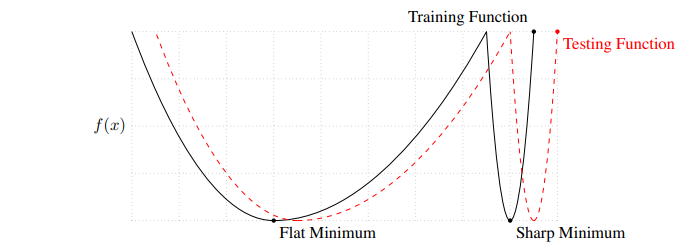
\includegraphics[scale=0.6]{assets/Keskar_et_al}\caption{\citep{keskar2016large} A Conceptual Sketch of Flat and Sharp Minima.
The Y-axis indicates value of the loss function and the X-axis the
weight space. }
\par\end{centering}
\end{figure}

\pagebreak{}

\subsection{Linear Neural Networks \label{subsec:Linear-Neural-Networks}}

Linear neural networks (LNN) are fully connected networks with no
neuron activation. The end-to-end function of a deep linear network
can always be rewritten as a shallow network, thus such networks do
not gain expressive power from increased depth, and will perform poorly
on complex real world problems. While it lacks important aspects of
modern neural network architectures, it is useful to appeal to the
simple case of linear models to see if there are parallel insights
that can help us better understand neural networks. Indeed under reasonable
assumptions their loss landscape is non-convex \citep{saxe2013exact}
and there exist \textquotedbl bad\textquotedbl{} saddle points (where
the Hessian has no negative eigenvalue) \citep{kawaguchi2016deep}.
Furthermore the training dynamics of gradient-flow on LNN show that
increased depth may implicitly accelerate optimization \citep{arora2018optimization},
exhibit incremental rank learning \citep{Arora2019Convrg} and is
implicitly biased towards minimal norm-like solutions \citep{yun2021a}.

\subsection{Main Results and Outline of the Paper}

The remainder of the paper is organized as follows. Section \ref{sec:Non-Singular-Problem-Setting}
describes the non-singular problem setting where a single end-to-end
solution exist. Section \ref{sec:Balancedness-of-Flattest} the notion
of \emph{balancedness} of flattest solutions, specifically it is shown
that not all flattest solutions are balanced (as defined in \citet{arora2018optimization}).
This inequivalence is shown under two different measures of minima
sharpness: maximal Hessian eigenvalue and Hessian trace. Section \ref{sec:singular-case}
extends the analysis of flattest minima, presented in \citep{Mulayoff2020Unique},
to setting where an infinitude of solutions exist. Section \ref{sec:Generalization-of-Flattest}
discusses the relationship between flatness and generalization. In
this section we provide a proof that generalization is indifferent
to flatness, in our settings. We prove this result under two different
settings: whitened data for the maximal Hessian eigenvalue measure,
and full rank label data for \emph{any} local flatness measure.

\section{Problem Setting}

Consider the case of linear regression: given a sample $S=\left(x^{(i)},y^{(i)}\right)_{i=1}^{N}\subseteq\left(\mathbb{R}^{d_{x}}\times\mathbb{R}^{d_{y}}\right),S\stackrel{i.i.d}{\sim}{\scriptstyle D^{N}}$.
Denote $X=\left(x^{(1)},x^{(2)},...,x^{(N)}\right)\in\mathbb{R}^{d_{x}\times N},Y=\left(y^{(1)},y^{(2)},...,y^{(N)}\right)\in\mathbb{R}^{d_{y}\times N}$,
our objective is to learn a linear transformation $f:\mathbb{R}^{d_{x}}\rightarrow\mathbb{R}^{d_{y}}$
corresponding to a matrix $W\in\mathbb{R}^{d_{y}\times d_{x}}$, that
minimizes the empirical (quadratic) loss: $L(W)=\left\Vert WX-Y\right\Vert _{F}^{2}$.
We study the overparameterized regime, in which $W$ is decomposed
as a product of matrices (LNN): $W_{i}\in\mathbb{R}^{d_{i}\times d_{i-1}},i\in\left[m\right]$
where $d_{0}:=d_{x},d_{N}:=d_{y}$. 

Denote $W_{1:m}:=\prod_{i=1}^{m}W_{i}$ ,the overparameterized objective
is defined by: 
\begin{equation}
\phi(W_{1},W_{2},...,W_{m})=L(W_{1:m})\label{eq:overparamloss}
\end{equation}

The set of global minima of $\phi$ is given by:
\begin{equation}
\Omega=\left\{ (W_{1},W_{2},...,W_{m})\in\prod_{i=1}^{m}\mathbb{R}^{d_{i}\times d_{i-1}}\ \Bigm\vert W_{1:m}\in\argmin_{T\in\mathbb{R}^{d_{y}\times d_{x}}}L(T)\right\} 
\end{equation}

\begin{defn}[Minima Flatness]
Denote the vectorization of the network's parameters $(W_{1},W_{2},...,W_{m})$.
Let $\omega:\prod_{i=1}^{m}\mathbb{R}^{d_{i}\times d_{i-1}}\rightarrow\mathbb{R}$
be some sharpness measure, then the set of \emph{flattest }global
minima is defined to be:
\begin{equation}
\Omega_{0}=\argmin_{w\in\Omega}\omega(W_{1},W_{2},...,W_{m})\label{eq:flattestmin}
\end{equation}

Where in (\ref{eq:flattestmin}) we have used a slight abuse of notation
by identifying $(W_{1},W_{2},...,W_{m})$ with $w$ for brevity.
\end{defn}
\newpage{}

\section{Balancedness of Flattest Solutions \label{sec:Balancedness-of-Flattest}}

As previously discussed SGD shows implicit bias towards flat solutions,
and is able to find generalizing solutions. Furthermore a variety
of optimization algorithms that explicitly bias towards flat solutions
achieve impressive performance \citep{izmailov2018averaging,chaudhari2019entropy,foret2021sharpnessaware}.
In light of this phenomena, one would expect that flat solutions are
in some sense regular, residing in benign regions where optimization
algorithms perform well.

Several works have showed a relationship between measures of flatness
and those of \textit{balancedness} ---a notion of scaling and alignment
between consecutive weight matrices--- \citep{Mulayoff2020Unique,ding2022flat}.
A particular definition of balancedness that is of interest in our
setting was proposed by \citet{arora2018optimization}: 
\begin{defn}[Balancedness]
\label{def:balancedness}For $\delta\ge0$ we say that the weight
matrices $\kaliseries W,m$ are $\delta-$balanced if:
\begin{equation}
\left\Vert W_{j+1}^{T}W_{j+1}-W_{j}W_{j}^{T}\right\Vert _{F}\le\delta\quad,\forall j\in[m-1]
\end{equation}

If $\kaliseries W,N$ are 0-balanced we simply say that they are balanced.
Let us denote the set of balanced weight matrices by:
\begin{equation}
\mathcal{B}=\left\{ (W_{1},W_{2},...,W_{m})\in\prod_{j=1}^{m}\mathbb{R}^{d_{i}\times d_{i-1}}\ \Bigm\vert\ W_{j+1}^{T}W_{j+1}=W_{j}W_{j}^{T}\quad,\forall j\in[m-1]\right\} 
\end{equation}

\medskip{}

A useful fact is that this notion of balancedness is conserved by
GF throughout optimization, formally:
\end{defn}
\begin{prop}[\citeauthor{Arora2019Convrg} ]
\label{prop:balancedness}Assume the weight matrices $\kaliseries W,m$
are initialized to be $\delta-\mathrm{balanced}$: 
\[
\left\Vert W_{j+1}^{T}(0)W_{j+1}(0)-W_{j}(0)W_{j}^{T}(0)\right\Vert _{F}\le\delta,\quad\forall j\in[m-1]
\]
 this property is conserved throughout optimization:
\[
\left\Vert W_{j+1}^{T}(t)W_{j+1}(t)-W_{j}(t)W_{j}^{T}(t)\right\Vert _{F}\le\delta,\quad\kaliForall j\in[m-1],\ t\ge0
\]
\end{prop}
We seek to refine the relationship between \ref{def:e2e-flatness}
and two common measures of flatness: maximal Hessian eigenvalue, and
the Hessian trace.

\subsection{Maximal Hessian Eigenvalue}

Let $H_{w}$ be the Hessian matrix of $\phi$ at the point $\left(\kaliseries W,m\right)$.
Define a sharpness measure $\omega:\prod_{i=1}^{m}\mathbb{R}^{d_{i}\times d_{i-1}}\rightarrow\mathbb{R}$
by:
\begin{equation}
\omega\left(\kaliseries W,m\right)=\lambda_{max}\left(H_{w}\right)\label{eq:max-hessian-eigenvalue}
\end{equation}

Note that this measure captures the sharpness of a point in the ``worst-case''
sense, and is the factor affecting stable convergence of GD and SGD
\citep{Mulayoff2020Unique,nar2018step}.

In particular they studied the case where a single end-to-end solution
exists:
\begin{enumerate}[label=\bfseries{C1}]
\item \label{assumption:nonsingular} The data's ambient dimension $d_{x}$
is smaller then the number of training samples $N$.
\end{enumerate}
In this case the unique solution can be written as $f^{\ast}(x)=Tx$
where: 
\begin{equation}
T=\hat{\Sigma}_{yx}\hat{\Sigma}_{x}^{-1}:=YX^{T}\left(XX^{T}\right)^{-1}
\end{equation}

We will deonte the the SVD of $T$ by:
\begin{equation}
T=USV^{T}
\end{equation}

\citep{Mulayoff2020Unique} showed that under the assumptions:
\begin{enumerate}[label=\bfseries{A\arabic{enumi}}]
\item  \label{assumption:capacity}The network has the capacity to implement
any linear function from $\mathbb{R}^{d_{x}}$ to $\mathbb{R}^{d_{y}}$:
$\min_{i\in\left[m\right]}\{d_{i}\}\ge\min\{d_{x},d_{y}\}.$
\item \label{assumption:white}The data is white, namely $\hat{\Sigma}_{x}=I_{d_{x}}$.
\end{enumerate}
The following sufficient condition for minima flatness holds:
\begin{thm}[Sufficient Condition, \citeauthor{Mulayoff2020Unique}]
\label{thm:sufficient}Assume (\ref{assumption:nonsingular}),(\ref{assumption:capacity}),(\ref{assumption:white}).
If a solution $w\in\Omega$ satisfies 
\[
\sigma_{\max}(W_{k})=\left(\sigma_{\max}\left(T\right)\right)^{\frac{1}{m}}
\]
 for all $k\in[m]$, then necessarily $w\in\Omega_{0}.$
\end{thm}
Using this fact it can be shown that GF starting from a balanced initialization
can only converge to flattest solutions. By \propref{balancedness}
we can see that any balanced solution $w\in\Omega\cap\mathcal{B}$
is in fact a flattest minima:
\begin{equation}
\Omega\cap\mathcal{B}\subseteq\Omega_{0}
\end{equation}

One may wonder if the reverse implication holds:
\begin{onehalfspace}
\begin{center}
\textit{Are all flattest solutions balanced? }
\par\end{center}
\end{onehalfspace}

The following proposition shows that this is not the case:
\begin{prop}
\label{prop:FlatUnbalanced}Assume (\ref{assumption:nonsingular}),(\ref{assumption:capacity}),(\ref{assumption:white})
and that $2\le\min\{d_{x},d_{y}\},m$. Unless $\sigma_{\min}\left(T\right)=\sigma_{\max}\left(T\right)$,
then there exists an unbalanced flattest solution, namely: 
\[
\Omega_{0}\nsubseteq\Omega\cap\mathcal{B}
\]
\end{prop}
\begin{proof}
[Proof sketch (proof in \ref{subsec:proof-flat-unbalanced})] We find
a flattest unbalanced solutions by ``perturbing'' the singular values
of consecutive weight matrices of a balanced solution: $\left(\kaliseries W,m\right)\in\Omega_{0}\cap\mathcal{B}$,
without changing its end-to-end function. 

As \citep{Mulayoff2020Unique} state, it is intractable to derive
a closed form expression for $\lambda_{\max}\left(H_{w}\right)$ at
an arbitrary minimum point, we therefore perturb the solution to meet
the conditions of \thmref{sufficient}.
\end{proof}
\begin{rem*}
Unfortunately the authors could not find such a perturbation for the
case of $\sigma_{\min}\left(T\right)=\sigma_{\max}\left(T\right)$
or find a more lenient sufficient condition.
\end{rem*}

\subsection{Hessian Trace}

The proof of $\text{\prettyref{prop:FlatUnbalanced}}$relied on the
fact that the maximal eigenvalue of the Hessian of $\phi$ is unaffected
by a small perturbation of the overparameterization non-maximal singular
values. The proof shows the ``worst case'' nature of this measure
(\ref{eq:max-hessian-eigenvalue}). We now study a different measure,
that depends on all of the overparameterization singular values: the
Hessian trace. Formally, define:

\begin{equation}
\omega\left(\kaliseries W,m\right)=Trace\left(H_{w}\right)\label{eq:sharp_def_trace}
\end{equation}

where $w$ is defined as $w:=Vec(W_{1},W_{2},...,W_{m})$ such that
$W_{m}\cdot...\cdot W_{1}=T$.

Next we revise the results of \citet{Mulayoff2020Unique} for the
trace measure.

\subsubsection{Sharpness of a general solution}
\begin{lem}
\label{lem:hes-trace}Assuming (\ref{assumption:nonsingular}) and
(\ref{assumption:white}), the trace of the Hessian for a solution
is:

\begin{equation}
Trace(H_{w})=2\sum_{k=1}^{m}||W_{k-1:1}||_{F}^{2}\cdot||W_{m:k+1}||_{F}^{2}\label{eq:hes-trace}
\end{equation}
\end{lem}
\begin{proof}
[Proof sketch (proof in \ref{subsec:proof-of-hes-trace})] 

We apply the trace function to the result from \citet{Mulayoff2020Unique}
for the Hessian structure, and using properties of Kronecker product
and trace, arrive to the result above.
\end{proof}

\subsubsection{Sharpness of a balanced solution}

Now, we discuss the case of a balanced solution:

\[
\forall i\in[m].W_{i}W_{i}^{T}=W_{i+1}^{T}W_{i+1}
\]

\begin{lem}
\label{lem:bal-hes-trace}For a balnced solution, it holds that: $||\prod_{i=k}^{n}W_{i}||_{F}^{2}=||S^{\frac{n-k+1}{m}}||_{F}^{2}$
where $W_{m:1}=T=USV^{T}$is the SVD of the End-to-End solution.
\end{lem}
\begin{proof}
From (\ref{subsec:proof-flat-unbalanced}) we know the following:
\[
U_{k}=V_{k+1},S_{k}=S_{k+1}
\]
 Thus we get that:
\[
\prod_{i=k}^{n}W_{i}=W_{n}W_{n-1}...W_{k+1}W_{k}=\mysvd n\mysvd{n-1}...\mysvd{k+1}\mysvd k=U_{n}S_{k}^{n-k+1}V_{k}^{T}
\]
 Comparing it with the end-to-end solution we get:
\[
U_{m}S_{1}^{m}V_{1}^{T}=W_{m:1}=T=USV^{T}=>\forall i\in[m].S_{i}=S^{\frac{1}{m}}
\]
 which yields:
\[
||\prod_{i=k}^{n}W_{i}||_{F}^{2}=||U_{n}S_{k}^{n-k+1}V_{k}^{T}||_{F}^{2}=||S^{\frac{n-k+1}{m}}||_{F}^{2}
\]

By using (\ref{lem:hes-trace}) with (\ref{eq:hes-trace}) we get
the following result for balanced solutions:

\begin{equation}
Trace(H_{w})=2\sum_{k=1}^{m}||S^{\frac{k-1}{m}}||_{F}^{2}\cdot||S^{\frac{m-k}{m}}||_{F}^{2}\label{eq:balanced_trace}
\end{equation}
\end{proof}

\subsection{Is balancedness equal to flattest solution?}

After revisiting \citet{Mulayoff2020Unique} with our new definition
for the sharpness of a solution, we can start and investigate if balancedness
equates to flatness of the solution.

We split this to 2 cases: the 2-Layer case, and the general m-layer
Case. As we will show, there is difference in the results, which stems
from the scaling of some elements in the equation (\ref{eq:hes-trace}).

\subsubsection{2-Layer case}

\paragraph{Non-Square Case\protect \\
}

In the non-square case, we have an issue of scaling: the trace has
a different scaling for each norm, thus providing us a way to find
a counter example.
\begin{lem}
\label{lem:non-square-case} Assume $T\in\mathbb{R}^{d_{X}\times d_{Y}}$
and $d_{X}\neq d_{Y}$. Then there exists a solution with lower sharpness
than any balanced solution.
\end{lem}
\begin{proof}
[Proof sketch (proof in \ref{subsec:proof-of-non-square-case})]

We bring a counter-example which has lower sharpness than the balanced
solution. As all balanced solutions have the same sharpness (by (\ref{eq:balanced_trace})),
we conclude that any balanced solution is not the flattest, and any
flattest solution is not balanced.
\end{proof}

\paragraph{Square Case\protect \\
}

In the square case, all the elements in (\ref{eq:hes-trace}) are
scales with the same constant - the dimension. Using this, we prove
that a solution is flattest if and only if the solution is balanced.
\begin{thm}
\label{thm:2-layer-case}Assume that $T=W_{2}W_{1}$ and $T\in\mathbb{R}^{d\times d}.$
Then a solution is flattest if and only if the solution is balanced.
\end{thm}
\begin{proof}
[Proof sketch (proof in \ref{subsec:proof-of-2-layer-case})]

First we show that balanced solution is always a flattest solution.

To show this we show that minimizing the trace of the hessian in the
2-Layer case for square end-to-end matrix is equal to the nuclear
norm of the end-to-end solution.

To show the other direction, that any flattest solution is indeed
balanced, we define a new function that achieves a local minima at
the solution. By differentiating this function and equating the derivative
to 0, we get the balancedness criterion defined in (\ref{def:balancedness}).
\end{proof}

\subsubsection{m-Layer Case}

As we saw before, the non-square case the statement is already invalid.
Thus we will focus here only on the square case.

We will show now that for the m-Layer case for $m\geq3$ balancedness
does not imply flattest solution, or vice versa.
\begin{lem}
\label{lem:m-layer-case} Assume $T\in\mathbb{R}^{d\times d}$ . Then
for $m>2$, there exists a solution $w=\left(W_{m},...W_{1}\right)$
with lower sharpness than any balanced solution.
\end{lem}
\begin{proof}
[Proof sketch (proof in \ref{subsec:proof-of-m-layer-case})]

We use a similar approach as in the proof of (\ref{lem:non-square-case}).
We build a counter example, and show that there exist a value for
the singular values of the end-to-end matrix, such that any balanced
solution will have a higher sharpness value than our counter example.
\end{proof}
In conclusion, we see that even the new definition of sharpness ((\ref{eq:sharp_def_trace}))
is not enough to achieve balancedness for the flattest solutions,
apart from the simple case of 2-layers.

\newpage{}

\section{Analysis of the Singular Case \label{sec:singular-case}}

\citeauthor{Mulayoff2020Unique} argued that in the singular case
any end-to-end solution has the same flatness, to this end they assumed
a single global minima exits (\ref{assumption:nonsingular}). We prove
their claim in \secref{Generalization-of-Flattest}, but first we
extend their analysis to the case where $n<d_{x}$ and multiple end-to-end
solutions exist. The results carry over naturally to the singular
case, and would later allow us to prove the aforementioned claim.

\subsection{Singular Problem Setting}

Define the set of end-to-end global minimizers by:

\begin{equation}
\Psi=\left\{ T\in\mathbb{R}^{d_{y}\times d_{x}}\ \Bigm\vert\ \in\argmin_{W\in\mathbb{R}^{d_{y}\times d_{x}}}L(W)\right\} 
\end{equation}

For a single end-to-end solution $T\in\mathbb{R}^{d_{y}\times d_{x}}$
we denote the set of overparameterizations as a LNN by:
\begin{equation}
\Omega(T)=\left\{ (W_{1},W_{2},...,W_{m})\in\prod_{i=1}^{m}\mathbb{R}^{d_{i}\times d_{i-1}}\ \Bigm\vert\ W_{1:m}=T\right\} 
\end{equation}

Define the sharpness of an overparameterization $\omega:\prod_{i=1}^{m}\mathbb{R}^{d_{i}\times d_{i-1}}\rightarrow\mathbb{R}$,
and of sharpness a solution $\rho:\mathbb{R}^{d_{y}\times d_{x}}\rightarrow\mathbb{R}$
respectively:

\begin{equation}
\omega(W_{1},W_{2},...,W_{m})=\lambda_{\mathrm{\max}}\left(H_{w}\right),\quad\rho(T)=\min_{(W_{1},W_{2},...,W_{m})\in\Omega(T)}\omega(W_{1},W_{2},...,W_{m})\label{def:e2e-flatness}
\end{equation}

Note that $\lambda_{\mathrm{\max}}\left(H_{w}\right)$ is continuous
in $w$ and that $\Omega(T)$ is closed in $\prod_{i=1}^{m}\mathbb{R}^{d_{i}\times d_{i-1}}$
so $\rho$ is well-defined.

We denote the set of flattest overparameterizations for a solution
$T$ by:
\[
\Omega_{0}(T)=\argmin_{(W_{1},W_{2},...,W_{m})\in\Omega(T)}\omega(W_{1},W_{2},...,W_{m})
\]

To study the connection between flatness and generalization one must
consider the singular case where more then one end-to-end solutions
exits ($N<d_{x}$ and the mapping is realizable) . In this case all
such solutions are given by:
\begin{equation}
\Psi=\left\{ YX^{+}+K\left(I_{d_{x}}-XX^{+}\right)\Bigm\vert K\in\mathbb{R}^{d_{y}\times d_{x}}\right\} \label{eq:singular-solutions}
\end{equation}

Where $\cdot^{+}$ is the Moore-Penrose pseudo-inverse.

Denote the set of flattest solutions by:
\begin{equation}
\Psi_{0}=\argmin_{T\in\Psi}\rho(T)
\end{equation}

We begin by examining a simplified version of the singular case, we
modify assumption (\ref{assumption:white}):
\begin{enumerate}[start=2, label=\bfseries{A\arabic{enumi}}]
\item \label{assumption:pseudo-white} The data is pseudo-white, namely
$\hat{\Sigma}_{x}=\begin{pmatrix}I_{N} & \mathbb{0}_{N\times\left(d_{x}-N\right)}\\
\mathbb{0}_{\left(d_{x}-N\right)\times N} & \mathbb{0}_{d_{x}-N}
\end{pmatrix}$.
\end{enumerate}
\begin{rem*}
We note that this assumption may be unreasonable for study of generalization.
Beside its inapplicability to modern practices, whitening is known
to potentially impede generalization ---mainly due to re-scaling
of feature variances \citep{wadia20whitening}. \citet{Mulayoff2020Unique}
conjectured that analogous result hold in the general setting, there
however, there seems to be no known closed form expression for $\lambda_{\mathrm{\max}}\left(H_{w}\right)$. 
\end{rem*}

\subsection{Extending the Analysis to the Singular Case}

We now extend \citeauthor{Mulayoff2020Unique} results to the singular
setting described in the previous section. 

First, note that lemma 2 (Hessian Structure) holds for any $(W_{1},W_{2},...,W_{m})\in\Omega(T)$,
$T\in\Psi$. 
\begin{thm}[Minimal Solution Sharpness]
 \label{thm:min-sharpness-singular}Assume (\ref{assumption:capacity}),
(\ref{assumption:pseudo-white}), then the minimal solution sharpness
is given by $\min_{T\in\Psi}\rho(T)=2m\left(\sigma_{\max}\left(YX^{T}\right)\right)^{2\left(1-\frac{1}{m}\right)}$,
i.e.: 
\[
\Psi_{0}=\left\{ T\in\Psi\ \Bigm\vert\ \in\rho(T)=2m\left(\sigma_{\max}\left(YX^{T}\right)\right)^{2\left(1-\frac{1}{m}\right)}\right\} 
\]
\end{thm}
The proof follows the scheme of the singular case \citep{Mulayoff2020Unique}: 
\begin{enumerate}
\item First we derive a uniform lower bound on the sharpness of an end-to-end
solution.
\item We show a solution which achieves this bound.
\end{enumerate}
\begin{lem}[Uniform Lower Bound]
\label{lemma:unif-lb}Let $T\in\Psi$ be a solution, define $\nu_{T}:\mathbb{R}^{d_{y}\times d_{x}}\rightarrow\mathbb{R}_{\ge0}$
by: 
\[
\nu_{T}\left(B\right)=2m\left\Vert \left(B\hat{\Sigma}_{x}^{\frac{1}{2}}T^{T}\right)^{m-1}B\hat{\Sigma}_{x}^{\frac{1}{2}}\right\Vert _{2}^{\frac{2}{m}}
\]
Then the following holds:
\begin{enumerate}[label=\Roman{enumi}.]
\item $\max_{\left\Vert B\right\Vert _{F}=1}\nu_{T}\left(B\right)\le\rho(T)$
. 
\item For the special case of \ref{assumption:pseudo-white}, $\forall T_{1},T_{2}\in\Psi.\max_{\left\Vert B\right\Vert _{F}=1}\nu_{T_{1}}\left(B\right)=\max_{\left\Vert B\right\Vert _{F}=1}\nu_{T_{2}}\left(B\right)=\rho(T)$,
namely:
\[
\rho(T)\ge2m\left(\sigma_{\max}\left(YX^{T}\right)\right)^{2\left(1-\frac{1}{m}\right)}\ ,\quad\forall T\in\Psi
\]
\end{enumerate}
\end{lem}
\begin{proof}
[Proof sketch (proof in \ref{subsec:proof-flat-unbalanced})] The
first part of the lemma proved in \citep{Mulayoff2020Unique}. Note
that $\max_{\left\Vert B\right\Vert _{F}=1}\nu_{T}\left(B\right)\le\rho(T)$
uniformly bounds all overparameterizations $w\in\Omega(T)$.

To see how the dependence on a specific end-to-end solution is dropped
in the section part, notice that for a solution $T=YX^{+}+K\left(I_{d_{x}}-XX^{+}\right)$:
\begin{align*}
\hat{\Sigma}_{x}^{\frac{1}{2}}T^{T} & =XX^{T}\left(\left(X^{T}\right)^{+}Y^{T}+\left(I_{d_{x}}-\left(X^{T}\right)^{+}X^{T}\right)K^{T}\right)\\
 & =X{\color{gray}\underset{=I_{N}}{\underbrace{{\normalcolor X^{T}\left(X^{T}\right)^{+}}}}}Y^{T}+X{\color{gray}\underset{=\mathbb{0}_{N\times d_{x}}}{\underbrace{{\normalcolor X^{T}\left(I_{d_{x}}-\left(X^{T}\right)^{+}X^{T}\right)}}}}K^{T}\\
 & =YX^{+}
\end{align*}

Where the third equality is due to to the properties of the pseudo-inverse
and that by (\ref{assumption:pseudo-white}) $X^{T}$ has linearly-independent
columns, thus $\left(X^{T}\right)^{+}$ is a left inverse.
\end{proof}
Next we show that there exist a solution that achieves this bound:
\begin{lem}
\label{lem:lower-bound-achieved}Assume (\ref{assumption:capacity}),(\ref{assumption:pseudo-white}).
There exists $T\in\Psi$ such that $\rho(T)=2m\left(\sigma_{\max}\left(YX^{T}\right)\right)^{2\left(1-\frac{1}{m}\right)}$.
\end{lem}
\textit{See proof in \ref{subsec:proof-of-lem-acheived}.}

\medskip{}

Using the necessary condition of \thmref{min-sharpness-singular},
we are able to derive a sufficient condition analogous to the non-singular
case (\thmref{sufficient}):
\begin{thm}[Sufficient Condition]
\label{thm:sufficient-singular}Assume (\ref{assumption:capacity}),(\ref{assumption:pseudo-white}).
If an overparameterization $w\in\varTheta(T)$ of a solution $T\in\Psi$
satisfies $\sigma_{\max}(W_{k})=\left(\sigma_{\max}\left(YX^{T}\right)\right)^{\frac{1}{m}}$
for all $k\in[m]$, then necessarily $w\in\Omega_{0}(T)$ and $T\in\Psi_{0}$.
\end{thm}
The proof of this theorem is analogous to the non-singular case in
\citep{Mulayoff2020Unique}, by using (\ref{thm:min-sharpness-singular}).

\pagebreak{}

\section{Generalization of Flattest Solutions \label{sec:Generalization-of-Flattest}}

\subsection{Motivation: Simple Linear Regression}

As discussed in sections \ref{subsec:Flatness-and-generalization},
\ref{subsec:Linear-Neural-Networks} it is not necessarily easy to
understand the source of generalization even for linear models. Before
studying the overparameterized setting, let us take a step back an
examine the case of simple underdetermined linear regression with
the quadratic loss: 
\[
L(W)=\left\Vert WX-Y\right\Vert _{F}^{2}
\]
In this setting the Hessian matrix of the loss function is given by:
\[
H_{L}(W)=I_{d_{y}\times d_{x}}\left(XX^{T}\right)^{\frac{1}{2}}\odot I_{d_{x}\times d_{y}}
\]

where $\odot$ denotes the Kronecker product.

Notice that the Hessian is independent of the choice of $W$, hence
any sharpness definition that depends only on it, cannot correlate
with generalization \label{subsec:reg-regression-indf}\citep{choromanska14surface}.

\citeauthor{Mulayoff2020Unique} claimed that a similar phenomena
holds in the overparameterized setting as-well, namely any end-to-end
solution has the same flatness, formally:
\begin{thm}
\label{thm:indifference}Assume (\ref{assumption:capacity}),(\ref{assumption:pseudo-white}).
All end-to-end solutions have the same flatness, namely: 
\[
\Psi=\Psi_{0}
\]
\end{thm}
Note that this claim is not trivial in the overparameterized setting,
as the Hessian is location dependent, and a closed form expression
for its top eigenvalue seems intractable.
\begin{lem}[Hessian Structure \citeauthor{Mulayoff2020Unique}]
\label{lem:-hessian-structure} Assume (\ref{assumption:capacity}).
If $w\in\Omega\left(T\right)$ and $T\in\Psi$ is a solution, then
\[
H_{w}=2\Phi\Phi^{T}
\]

where $\Phi=\left[\kaliseries{\Phi^{T}},m\right]^{T}$, with 
\[
\Phi_{k}=\left(W_{k-1:1}\hat{\Sigma}_{x}^{\frac{1}{2}}\right)\odot\left(W_{m:k+1}\right)^{T}
\]
\end{lem}
The Hessian structure provides intuition for (\ref{thm:indifference}):
note that $\Phi_{k}$ is a $d_{k}d_{k-1}\times d_{x}d_{y}$ matrix,
therefore $\Phi$ is a $P\times d_{x}d_{y}$ where $P=\sum_{k=1}^{m}d_{k}d_{k-1}$
is the total number of parameters in the network. This shows that
for networks with more than one layer the Hessian at an end-to-end
solution is rank-deficient. Formally, by (\ref{lem:-hessian-structure})
if $w\in\Omega(T)$ and $T\in\Psi$ then $H_{w}$ is a $P\times P$
matrix, and $rank\left(H_{w}\right)\le d_{x}d_{y}<P^{2}$.

\subsection{Proof Outline for Theorem \ref{thm:indifference}}

We begin by showing that if a point $w\in\Theta(T_{1})$ at the overparameterized
space satisfies a certain regularity constraint (\ref{eq:overparam-regularity}),
then for every other $T_{2}\in\mathbb{R}^{d_{y}\times d_{x}}$ such
that $\left(T_{2}-T_{1}\right)X=0$, there exists a direction $\bar{w}$
in the overparameterized space, that connects $\Theta(T_{1})$ with
$\Theta(T_{2})$, along which $\phi$ is constant.
\begin{prop}[Invariant Directions]
\label{prop:invariant-directions}Assuming \ref{assumption:capacity}
let $T_{1},T_{2}\in\mathbb{R}^{d_{y}\times d_{x}}$ such that $\left(T_{2}-T_{1}\right)X=0$.
Assume $T_{1}$ admits an overparameterization \textup{$\left(\kaliseries{\bar{W}},m\right)\in\varTheta(T_{1})$
such that: 
\begin{equation}
rank\left(\bar{W}_{2:m}\right)=d_{y}\ or\ rank\left(\bar{W}_{1:m-1}\right)=d_{x}\label{eq:overparam-regularity}
\end{equation}
 then} there exists a direction $\left(\Delta_{1},\Delta_{2},...,\Delta_{m}\right)\in\prod_{i=1}^{m}\mathbb{R}^{d_{i}\times d_{i-1}}$
such that: 
\begin{enumerate}[label=\alph{enumi}]
\item $T_{2}=\left(\bar{W}_{i}+\Delta_{i}\right)_{1:m}$
\item The overparameterized loss is constant along $\left(\Delta_{1},\Delta_{2},...,\Delta_{m}\right),$
namely: 
\[
\phi\left(\left(\kaliseries{\bar{W}},m\right)+t\left(\Delta_{1},\Delta_{2},...,\Delta_{m}\right)\right)=\phi\left(\kaliseries{\bar{W}},m\right)\ ,\ \forall t\in\mathbb{R}
\]
\end{enumerate}
\end{prop}
\begin{proof}
Assume $d_{y}\le d_{x}$, define $\left(\Delta_{1},\Delta_{2},...,\Delta_{m}\right)\in\prod_{i=1}^{m}\mathbb{R}^{d_{i}\times d_{i-1}}$
by:
\begin{equation}
\Delta_{1}=\left(\bar{W}_{2:m}\right)^{+}\left(T_{2}-T_{1}\right)\ ,\quad\Delta_{i}=\mathbb{0}_{d_{i}\times d_{i-1}},i\in\left\{ 2,3,...,m\right\} \label{def:dead-direction-delta}
\end{equation}

Notice that by construction $\left(\Delta_{1},\Delta_{2},...,\Delta_{m}\right)$
shifts $\left(\kaliseries{\bar{W}},m\right)$ to $\varTheta(T_{1}),$i.e.:
\[
\left(\bar{W}_{i}+\Delta_{i}\right)_{1:m}=\bar{W}_{2:m}\left(\bar{W}_{1}+\left(\bar{W}_{2:m}\right)^{+}\left(T_{2}-T_{1}\right)\right)=T_{2}
\]

Where the last equality holds because by assumption $\bar{W}_{2:m}$
has linearly-independent rows, so $\left(\bar{W}_{2:m}\right)^{+}$
is a right inverse.

Next we show that the loss is constant along $\left(\Delta_{1},\Delta_{2},...,\Delta_{m}\right)$:
\begin{align*}
\phi\left(\left(\kaliseries{\bar{W}},m\right)+t\left(\Delta_{1},\Delta_{2},...,\Delta_{m}\right)\right) & =\left\Vert \left(\bar{W}_{i}+t\Delta_{i}\right)_{1:m}X-Y\right\Vert _{F}^{2}\\
 & =\left\Vert \bar{W}_{2:m}\left(\bar{W}_{1}+t\left(\bar{W}_{2:m}\right)^{+}\left(T_{2}-T_{1}\right)\right)X-Y\right\Vert _{F}^{2}\\
 & =\left\Vert \bar{W}_{1:m}X+t\bar{W}_{2:m}\left(\bar{W}_{2:m}\right)^{+}\left(T_{2}-T_{1}\right)X-Y\right\Vert _{F}^{2}\\
 & =\left\Vert \bar{W}_{1:m}X-Y\right\Vert _{F}^{2}\\
 & =\phi\left(\kaliseries{\bar{W}},m\right)
\end{align*}

Where in the third equality we used the assumption $\left(T_{2}-T_{1}\right)X=0$.

For the case where $d_{x}<d_{y}$ we can similarly define:
\[
\Delta_{m}=\left(\bar{W}_{1:m-1}\right)^{+}\left(T_{2}-T_{1}\right)\ ,\quad\Delta_{i}=\mathbb{0}_{d_{i}\times d_{i-1}},i\in\left[m-1\right]
\]

In this case $W_{1:m-1}$ has linearly-independent columns, so $\left(W_{1:m-1}\right)^{+}$
is a left inverse, the proof is analogous.
\end{proof}
\begin{cor}
\label{cor:dead-direction-local}Under the assumptions and notations
of \propref{invariant-directions}, there exists a direction $\left(\Delta_{1},\Delta_{2},...,\Delta_{m}\right)\in\prod_{i=1}^{m}\mathbb{R}^{d_{i}\times d_{i-1}}$
such that:
\begin{enumerate}
\item $T_{2}=\left(\bar{W}_{i}+\Delta_{i}\right)_{1:m}$
\item The overparameterized loss $\phi$ is locally constant along $\left(\Delta_{1},\Delta_{2},...,\Delta_{m}\right)$.
Formally define the translation function:
\[
s_{t}:\prod_{i=1}^{m}\mathbb{R}^{d_{i}\times d_{i-1}}\rightarrow\prod_{i=1}^{m}\mathbb{R}^{d_{i}\times d_{i-1}},\quad s(W_{1},W_{2},...,W_{m})=(W_{1},W_{2},...,W_{m})+t\left(\Delta_{1},\Delta_{2},...,\Delta_{m}\right)
\]
then there exist $\varepsilon>0$ such that:
\[
\forall t\in\mathbb{R}.\ \phi|_{B\left((\bar{W}_{1},\bar{W}_{2},...,\bar{W}_{m}),\varepsilon\right)}\equiv\phi\circ s_{t}|_{B\left((\bar{W}_{1},\bar{W}_{2},...,\bar{W}_{m}),\varepsilon\right)}
\]
\end{enumerate}
\end{cor}
\corref{dead-direction-local} provides an lower bounds the sharpness
of \textit{all }\textit{\emph{solutions $T\in\Psi$ by the sharpness
of a solution $T_{0}$ that admits (\ref{eq:overparam-regularity}).
Thus to prove the theorem, it is suffices to show the existence of
a }}\textit{flattest}\textit{\emph{ solution $T_{0}\in\Psi_{0}$ that
admits (\ref{eq:overparam-regularity}).}}
\begin{rem*}
Note that while \corref{dead-direction-local} holds for any local
definition of sharpness $\omega$, the existence of such a flattest
solution may depend on the specific definition. In section \subsecref{def-agnostic-indf}
we provide a definition-agnostic proof, under different assumptions. 
\end{rem*}
\begin{lem}
\label{lem:existence-of-fr}Assuming (\ref{assumption:capacity}),(\ref{assumption:pseudo-white}).
There exists $T_{0}\in\Psi_{0}$ that admits a flattest overparameterization
\textup{$(W_{1},W_{2},...,W_{m})\in\varTheta_{0}(T_{0})$ such that:
\[
rank\left(\bar{W}_{2:m}\right)=d_{y}\ or\ rank\left(\bar{W}_{1:m-1}\right)=d_{x}
\]
}
\end{lem}
\begin{proof}
[Proof sketch (proof in \ref{subsec:proof-of-ex-of-frs})]The proof
follows a similar argument as in \propref{FlatUnbalanced}. Let $\left(W_{1}^{\ast},W_{2}^{\ast},...,W_{m}^{\ast}\right)$
be the canonical overparameterization of $T_{0}$. We define a new
overparameterization $\left(W_{1},W_{2},...,W_{m}\right)$ by ``perturbing''
the singular values of each weight matrix $W_{j}^{\ast}$ for $2\le j\le m$
into non-singularity. Because $\left(W_{1}^{\ast},W_{2}^{\ast},...,W_{m}^{\ast}\right)$
are balanced this perturbation does not change the end-to-end function.
By \thmref{sufficient-singular}, for a sufficiently small perturbation,
$\left(W_{1},W_{2},...,W_{m}\right)$ is a flattest overparameterization
of $T_{0}$.
\end{proof}

\subsubsection*{Completing the Proof of Theorem \ref{thm:indifference}}

We show the case where $d_{y}\le d_{x}$, the case of $d_{x}<d_{y}$
is analogous. 

By \lemref{existence-of-fr} we know that there exists $T_{0}\in\Psi_{0}$
that admits an overparameterization $(U_{1},U_{2},...,U_{m})\in\varTheta(T_{0})$
such that $rank\left(W_{2:m}\right)=d_{y}$.

Let $T'\in\Psi$ be a solution, and $(W'_{1},W'_{2},...,W'_{m})\in\varTheta(T')$
an overparameterization of it, by \corref{dead-direction-local} for
\[
\Delta_{1}=\left(W_{2:m}\right)^{+}\left(T_{2}-T_{1}\right)\ ,\quad\Delta_{i}=\mathbb{0}_{d_{i}\times d_{i-1}},i\in\left\{ 2,3,...,m\right\} 
\]
it holds that:
\begin{enumerate}
\item $(U_{1},U_{2},...,U_{m})+(\Delta_{1},\Delta_{2},...,\Delta_{m})\in\varTheta(T')$
\item $\exists\varepsilon>0.\ \phi|_{B\left((U_{1},U_{2},...,U_{m}),\varepsilon\right)}\equiv\phi\circ s_{1}|_{B\left((\bar{W}_{1},\bar{W}_{2},...,\bar{W}_{m}),\varepsilon\right)}$
\end{enumerate}
Because $\phi$ is locally identical in a neighborhood of $(U_{1},U_{2},...,U_{m})$
and of $(U_{1}+\Delta_{1},U_{2}+\Delta_{2},...,U_{m}+\Delta_{m})$,
it particularly holds that: 
\begin{equation}
H_{\phi}(U_{1},U_{2},...,U_{m})=H_{\phi}(U_{1}+\Delta_{1},U_{2}+\Delta_{2},...,U_{m}+\Delta_{m})
\end{equation}

and specifically:
\[
\rho\left(T'\right)\stackrel{\ref{eq:petubation-between-e2e}}{\le}\lambda_{\max}\left(H_{\phi}(U_{1}+\Delta_{1},U_{2}+\Delta_{2},...,U_{m}+\Delta_{m})\right)=\lambda_{\mathrm{\max}}\left(H_{\phi}(U_{1},U_{2},...,U_{m})\right)=2m\left(\sigma_{\max}\left(YX^{T}\right)\right)^{2\left(1-\frac{1}{m}\right)}
\]

Now by \thmref{sufficient-singular}: $2m\left(\sigma_{\max}\left(YX^{T}\right)\right)^{2\left(1-\frac{1}{m}\right)}\le\rho\left(T'\right)$,
hence:
\[
T'\in\Psi_{0}
\]


\subsection{\label{subsec:def-agnostic-indf}Invariance Under Any Local Measure}

As discussed in \ref{sec:Balancedness-of-Flattest} there are many
different definitions for the sharpness of a solutions. 

The proof of \lemref{existence-of-fr} relied on tolerance of the
maximal Hessian eigenvalue to small perturbations of singular values,
this begs the question:
\begin{onehalfspace}
\begin{center}
\textit{Is there a definition of sharpness under which not all solutions
are flattest?}
\par\end{center}
\end{onehalfspace}

The following corollary of \corref{dead-direction-local} shows that
under the assumption that $d_{y}\le n\le d_{x}$ and that $rank(Y)=d_{y}$
(as is usually the case in deep learning), any sharpness measure $\omega:\prod_{i=1}^{m}\mathbb{R}^{d_{i}\times d_{i-1}}\rightarrow\mathbb{R}$
that depends only on a local neighborhood of $\phi$ does not correlate
with generalization.
\begin{thm}
Assume that that $d_{y}\le N\le d_{x}$, $rank(Y)=d_{y}$ and $rank(X)=N$.
Let $\omega:\prod_{i=1}^{m}\mathbb{R}^{d_{i}\times d_{i-1}}\rightarrow\mathbb{R}$
be a sharpness measure such that:
\[
\forall w,u\in\prod_{i=1}^{m}\mathbb{R}^{d_{i}\times d_{i-1}}.\left(\exists\varepsilon>0.\ \phi\left(B\left(w,\varepsilon\right)\right)=\phi\left(B\left(u,\varepsilon\right)\right)\right)\rightarrow\omega(w)=\omega(u)
\]

then any end-to-end solution is a flattest solution in the sense of
$\rho$, namely: $\Psi=\Psi_{0}$.
\end{thm}
\begin{proof}
By our assumption for any solution $T\in\Psi$ it holds that $rank\left(T\right)\ge rank\left(TX\right)=rank\left(Y\right)=d_{y}$.
Specifically this holds for any flattest solution $T_{0}\in\Psi_{0}$,
thus if $\left(\kaliseries W,m\right)\in\varTheta_{0}\left(T_{0}\right)$
is a flattest overparameterization, it holds that $rank\left(W_{2:m}\right)\ge rank\left(T_{0}\right)=d_{y}$.

Let $T'\in\Psi$ be a solution, by \corref{dead-direction-local}
we know that there exists $\left(\kaliseries{W'},m\right)\in\varTheta\left(T'\right)$
and $\varepsilon>0$ such that:
\[
\phi\left(B\left(\left(\kaliseries{\bar{W}},m\right),\varepsilon\right)\right)=\phi\left(B\left(\left(\kaliseries{W'},m\right),\varepsilon\right)\right)
\]

therefore by the locality of $\omega$:
\[
\min_{T\in\Psi}\rho\left(T\right)=\rho\left(T_{0}\right)=\omega\left(\kaliseries{\bar{W}},m\right)=\omega\left(\kaliseries{W'},m\right)\ge\rho\left(T'\right)
\]

thus we conclude that $T'\in\Psi_{0}.$
\end{proof}
\newpage\printbibliography

\newpage{}

\appendix

\section{Deferred Proofs}

\subsection{\label{subsec:proof-flat-unbalanced}Proof of Proposition \ref{prop:FlatUnbalanced}}
\begin{proof}
First, notice that the set $\Omega_{0}\cap\mathcal{B}$ is non-empty.
Mulayoff et al. (2020) proposed the canonical flattest solution:
\begin{equation}
W_{m}^{\ast}=US_{m}^{\frac{1}{m}},\quad W_{j}^{\ast}=S_{j}^{\frac{1}{m}},\quad W_{1}^{\ast}=S_{1}^{\frac{1}{m}}V^{T}\label{eq:Cannonical-sol}
\end{equation}

Where $S_{j}$ is used to denote the $d_{j}\times d_{j-1}$ matrix
whose $k$th diagonal entry is $\sigma_{k}\left(T\right)$ and $\sigma_{k}\left(T\right)$
is the $k$th largest singular value of $T$. By \thmref{sufficient}
this is indeed a flattest solution, and one can readily see that it
is also balanced.

Now let $\left(\kaliseries W,m\right)\in\Omega_{0}\cap\mathcal{B}$
be a flattest balanced solution which satisfies the sufficient condition
in \thmref{sufficient}, we transform it into an unbalanced flattest
solution.

Let $k\in\left[m-1\right]$ and denote the SVD decomposition of $W_{k},\;W_{k+1}$
by: 
\[
W_{k}=U_{k}S_{k}V_{k}^{T},\;W_{k+1}=U_{k+1}S_{k+1}V_{k+1}^{T}
\]

Without loss of generality, assume that the elements along the main
diagonal of $S_{k}$ are decreasing.

Because $w$ is balanced we know that: $V_{k+1}S_{k+1}^{2}V_{k+1}^{T}=U_{k}S_{k}^{2}U_{k}^{T}$ 

For a given $k$, the two sides of the above equation are both orthogonal
eigenvalue decompositions of the same matrix. Denote its eigenvalues
by $\lambda_{1}^{k},...,\lambda_{r_{k}}^{k}$and the multiplicity
of the $i$th eigenvalue by $\mu_{i}^{k}$, there exists orthogonal
matrices $O_{k,i}\in\mathbb{R}^{\mu_{i}\times\mu_{i}}$ such that:

\begin{equation}
U_{k}=V_{k+1}\cdot diag\left(O_{k,1},...,O_{k,r_{k}}\right),\quad S_{k}=S_{k+1}\label{eq:SvdChain}
\end{equation}

$O_{k,i}$ here is simply a matrix changing between orthonormal bases
of the eigenspace of $\lambda_{i}^{k}$.

We create a flattest unbalanced solution by ``perturbing'' $w$:

\medskip{}
\begin{elabeling}{00.00.0000}
\item [{\uline{If\ \mbox{$\exists l\in[r].0<\sigma_{l}^{(k)}<\left(\sigma_{\max}\left(T\right)\right)^{\frac{1}{m}}$}:}}] Let
$\varepsilon>0$ such that $\left(1+\epsilon\right)\sigma_{l}^{(k)}\le\left(\sigma_{\max}\left(T\right)\right)^{\frac{1}{m}}$,
define $\bar{S}_{k+1},\bar{S}_{k}$ by:
\[
\left(\bar{S}_{k}\right)_{i,j}=\begin{cases}
\left(S_{k}\right)_{i,j} & (i,j)\neq(l,l)\\
\frac{\sigma_{l}^{(k)}}{1+\varepsilon} & (i,j)=(l,l)
\end{cases}\;,\left(\bar{S}_{k+1}\right)=\begin{cases}
\left(S_{k+1}\right)_{i,j} & (i,j)\neq(l,l)\\
\left(1+\varepsilon\right)\sigma_{2}^{(k)} & (i,j)=(l,l)
\end{cases}
\]
\[
\bar{W}_{k}=U_{k}\bar{S}_{k}V_{k}^{T},\;\bar{W}_{k+1}=U_{k+1}\bar{S}_{k+1}\left(V_{k+1}\cdot diag\left(O_{k,1},...,O_{k,r_{k}}\right)\right)^{T}
\]
 We define $\bar{W}_{j}=W_{j}$ for $j\in\left[m\right]\backslash\left\{ k,k+1\right\} $
and $\bar{w}=vec\left(\kaliseries{\bar{W}},m\right)$, by (\ref{eq:SvdChain})
we have:
\begin{align*}
\bar{W}_{1:m} & =\prod_{j=k+2}^{m}W_{j}U_{k+1}\bar{S}_{k+1}{\color{gray}\underset{=I_{d_{k}}}{\underbrace{{\normalcolor \left(V_{k}\cdot diag\left(O_{k,1},...,O_{k,r_{k}}\right)\right)^{T}U_{k}}}}}\bar{S}_{k}V_{k}^{T}\prod_{j=1}^{k-1}W_{j}\\
 & =\prod_{j=k+2}^{m}W_{j}{\color{gray}\underset{\overset{\eqref{eq:SvdChain}}{=}W_{k+1}W_{k}}{\underbrace{{\normalcolor U_{k+1}\left(S_{k}^{2}\right)V_{k}^{T}}}}}W_{k+1}\prod_{j=1}^{k-1}W_{j}\\
 & =W_{1:m}=T\\
 & \Rightarrow\bar{W}_{1:m}\in\Omega
\end{align*}
 It remains to notice that by \thmref{sufficient} $\bar{w}\in\Omega_{0}$
and by the contra-positive of (\ref{eq:SvdChain}) $\bar{w}$ is not
balanced.
\item [{\uline{If\ \mbox{$\sigma_{2}^{(k)}=\sigma_{3}^{(k)}=\dotsc=\sigma_{r}^{(k)}=0$}:}}] We
define a flattest unbalanced solution in a similar fashion:
\[
\left(\bar{S}_{k+1}\right)=\begin{cases}
\left(S_{k+1}\right)_{i,j} & (i,j)\neq(2,2)\\
\frac{\left(\sigma_{\max}\left(T\right)\right)^{\frac{1}{m}}}{2} & (i,j)=(2,2)
\end{cases}\;,\quad\bar{W}_{k+1}=U_{k+1}\bar{S}_{k+1}\left(V_{k+1}\cdot diag\left(O_{k,1},...,O_{k,r_{k}}\right)\right)
\]
The results follows using the same arguments as for the case of $\sigma_{2}^{(k)}>0$.
\item [{\uline{If\ \mbox{$\forall\left(\kaliseries W,m\right)\in\left(\Omega_{0}\cap\mathcal{B}\right).$}\mbox{$\forall k\in[m].\sigma_{1}^{(k)}\ge\sigma_{2}^{(k)}\ge\dotsc\ge\sigma_{r}^{(k)}\ge\left(\sigma_{\max}\left(T\right)\right)^{\frac{1}{m}}:$}}}]~
\begin{elabeling}{00.00.0000}
\item [{If\ $\exists\left(\kaliseries W,m\right)\in\left(\Omega_{0}\cap\mathcal{B}\right).$$\exists k\in[m].\sigma_{1}^{(k)}>\left(\sigma_{\max}\left(T\right)\right)^{\frac{1}{m}}$:}]~
\begin{elabeling}{00.00.0000}
\item [{If\ $\forall k\in[m],l\in[rank\left(W_{k}\right)].\ \sigma_{l}^{(k)}>\left(\sigma_{k}\left(T\right)\right)^{\frac{1}{m}}\rightarrow u_{l}^{(k)}\in Ker\left(W_{k+1:m}\right)$:}] We
can decrease all such singular values to $\left(\sigma_{k}\left(T\right)\right)^{\frac{1}{m}}$
(and even 0), without changing the end-to-end solution: $W_{1:m}$.
Denote the perturbed solution by $\left(\kaliseries{\bar{W}},m\right)$
we show by induction on $k\in[m]$ that $\bar{W}_{1:m}x=\bar{W}_{k+1:m}W_{1:k}x$
for $x\in Im(X).$
\begin{elabeling}{00.00.0000}
\item [{Induction\ Base\ (k=1):}] W.L.O.G we assume that only $\sigma_{l}^{(1)}>\left(\sigma_{\max}\left(T\right)\right)^{\frac{1}{m}}$:
\end{elabeling}
\begin{alignat*}{1}
\bar{W}_{1:m}x & =\bar{W}_{2:m}\left(\sigma_{l}^{(1)}\left\langle x,v_{l}^{(1)}\right\rangle u_{l}^{(1)}+\sum_{l\neq i\in[d_{x}]}\sigma_{i}^{(1)}\left\langle x,v_{i}^{(1)}\right\rangle u_{i}^{(1)}\right)\\
 & \stackrel{}{=}\bar{W}_{2:m}\left(\sum_{l\neq i\in[d_{x}]}\sigma_{i}^{(1)}\left\langle x,v_{i}^{(1)}\right\rangle u_{i}^{(1)}\right)\\
 & =\bar{W}_{2:m}\left(\sum_{l\neq i\in[d_{x}]}\sigma_{i}^{(1)}\left\langle x,v_{i}^{(1)}\right\rangle u_{i}^{(1)}\right)=\bar{W}_{2:m}W_{1}x
\end{alignat*}

\begin{elabeling}{00.00.0000}
\item [{Induction\ step:}] Assume that the claim holds for all $a\in[k]$,
again w.l.o.g assume that only $\sigma_{l}^{(k+1)}>\left(\sigma_{\max}\left(T\right)\right)^{\frac{1}{m}}$.
\begin{alignat*}{1}
\bar{W}_{1:m}x & =\bar{W}_{k+1:m}\left(\sigma_{i}^{(k)}\left\langle \bar{W}_{1:k-1}x,v_{l}^{(k)}\right\rangle u_{l}^{(k)}+\sum_{l\neq i\in[d_{x}]}\sigma_{i}^{(k)}\left\langle \bar{W}_{1:k-1}x,v_{i}^{(k)}\right\rangle u_{i}^{(k)}\right)\\
 & \stackrel{i.h.}{=}\bar{W}_{k+1:m}\left(\sum_{l\neq i\in[d_{x}]}\sigma_{i}^{(k)}\left\langle W_{1:k-1}x,v_{i}^{(k)}\right\rangle u_{i}^{(k)}\right)=\bar{W}_{k+2:m}W_{1:k+1}x
\end{alignat*}
\end{elabeling}
Thus $\left(\kaliseries{\bar{W}},m\right)\in\left(\Omega\cap\mathcal{B}^{C}\right),$and
by \thmref{sufficient} $\left(\kaliseries{\bar{W}},m\right)\in\Omega_{0}$.
\end{elabeling}
Assume by contradiction that $\exists k\in[m],l\in[r_{k}].\ \sigma_{l}^{(k)}>\left(\sigma_{k}\left(T\right)\right)^{\frac{1}{m}}\wedge u_{l}^{(k)}\notin Ker\left(W_{k+1:m}\right)$.

If $u_{l}^{(k)}\notin W_{1:k-1}X$ we can set $\sigma_{l}^{(k)}=\left(\sigma_{k}\left(T\right)\right)^{\frac{1}{m}}$
and using a similar induction we show that the perturbed end-to-end
matrix is a solution.

Otherwise, we know that $\exists x\in Im\left(X\right).W_{1:k-1}x=u_{l}^{(k)}$.
Notice that: 
\[
\sigma_{\min}\left(W_{k+1:m}\right)\ge\prod_{j=k+1}^{m}\sigma_{\min}^{(j)}\ge\left(\sigma_{\max}\left(T\right)\right)^{\frac{m-k+1}{m}},\quad\sigma_{\min}\left(W_{1:k-1}\right)\ge\prod_{j=1}^{k-1}\sigma_{\min}^{(j)}\ge\left(\sigma_{\max}\left(T\right)\right)^{\frac{k-1}{m}}
\]
\begin{align*}
\Rightarrow\sigma_{\max}\left(T\right)\left\Vert x\right\Vert _{2} & \ge\left\Vert W_{1:m}x\right\Vert \\
 & \ge\left(\sigma_{\max}\left(T\right)\right)^{\frac{k-1}{m}}\sigma_{l}^{(k)}\left\Vert W_{k+1:m}u_{l}^{(k)}\right\Vert _{2}\left\Vert x\right\Vert _{2}\\
 & \ge\left(\sigma_{\max}\left(T\right)\right)^{\frac{m-1}{m}}\sigma_{l}^{(k)}\left\Vert x\right\Vert _{2}\\
 & >\sigma_{\max}\left(T\right)\left\Vert x\right\Vert _{2}
\end{align*}

where the first inequality is true because the $l_{2}$ operator norm
is induced.
\end{elabeling}
\end{elabeling}
\end{proof}
%

\subsection{\label{subsec:proof-of-hes-trace}Proof of Lemma \ref{lem:hes-trace}}
\begin{proof}
Following Mulayoff et.al. (2020), we know that the hessian at a global
minimum has the following form:

\[
H_{w}=2\Phi\Phi^{T}
\]
\[
\Phi=\left[\Phi_{1}^{T},\Phi_{2}^{T},...,\Phi_{m}^{T}\right]{}^{T}
\]
\[
\Phi_{k}=\left(\prod_{j=1}^{k-1}W_{j}\Sigma_{x}^{0.5}\right)\odot\left(\prod_{i=k+1}^{m}W_{i}\right)^{T}
\]

Where $\odot$ is the kronecker product.

Thus we get the follwing:

\[
Sharp(w)=Trace(H_{w})=Trace(2\Phi\Phi^{T})=2\sum_{i=1}^{m}Trace(\Phi_{i}\Phi_{i}^{T})
\]
\begin{alignat}{1}
Trace(\Phi_{i}\Phi_{i}^{T}) & =Trace\left(\left[\left(\prod_{j=1}^{k-1}W_{j}\Sigma_{x}^{0.5}\right)\odot\left(\prod_{i=k+1}^{m}W_{i}\right)^{T}\right]\left[\left(\prod_{j=1}^{k-1}W_{j}\Sigma_{x}^{0.5}\right)\odot\left(\prod_{i=k+1}^{m}W_{i}\right)^{T}\right]^{T}\right)\nonumber \\
 & =Trace\left(\left[\left(\prod_{j=1}^{k-1}W_{j}\Sigma_{x}^{0.5}\right)\odot\left(\prod_{i=k+1}^{m}W_{i}\right)^{T}\right]\left[\left(\prod_{j=1}^{k-1}W_{j}\Sigma_{x}^{0.5}\right)^{T}\odot\left(\prod_{i=k+1}^{m}W_{i}\right)\right]\right)\label{eq:trace}\\
 & =Trace\left(\left[\left(\prod_{j=1}^{k-1}W_{j}\Sigma_{x}^{0.5}\right)\left(\prod_{j=1}^{k-1}W_{j}\Sigma_{x}^{0.5}\right)^{T}\right]\odot\left[\left(\prod_{i=k+1}^{m}W_{i}\right)^{T}\left(\prod_{i=k+1}^{m}W_{i}\right)\right]\right)\nonumber \\
 & =Trace\left(\left(\prod_{j=1}^{k-1}W_{j}\Sigma_{x}^{0.5}\right)\left(\prod_{j=1}^{k-1}W_{j}\Sigma_{x}^{0.5}\right)^{T}\right)\cdot Trace\left(\left(\prod_{i=k+1}^{m}W_{i}\right)^{T}\left(\prod_{i=k+1}^{m}W_{i}\right)\right)\nonumber \\
 & =||\prod_{j=1}^{k-1}W_{j}\Sigma_{x}^{0.5}||_{F}^{2}\cdot||\prod_{i=k+1}^{m}W_{i}||_{F}^{2}\nonumber 
\end{alignat}
 

By our assumption, $\Sigma_{x}^{-1}=Id$, turning (\ref{eq:trace})
into:

\begin{equation}
Trace(\Phi_{i}\Phi_{i}^{T})=||\prod_{j=1}^{k-1}W_{j}||_{F}^{2}\cdot||\prod_{i=k+1}^{m}W_{i}||_{F}^{2}=||W_{k-1:1}||_{F}^{2}\cdot||W_{m:k+1}||_{F}^{2}\label{eq:trace2}
\end{equation}

Where we used the following notation:

\begin{alignat*}{1}
W_{n:k} & :=\prod_{i=k}^{n}W_{i}=W_{n}W_{n-1}...W_{k}
\end{alignat*}

Using (\ref{eq:trace2}) we get the following:

\[
Trace(H_{w})=2\sum_{k=1}^{m}||W_{k-1:1}||_{F}^{2}\cdot||W_{m:k+1}||_{F}^{2}
\]
\end{proof}

\subsection{\label{subsec:proof-of-non-square-case}Proof of Lemma (\ref{lem:non-square-case})}
\begin{proof}
Let $T=USV^{T}\in\mathbb{R}^{d_{X}\times d_{Y}}$ be the SVD decomposition,
where: 
\[
S=\left[\begin{array}{ccccc}
x & 0 & \cdots & \cdots & 0\\
0 & 1 & \ddots &  & \vdots\\
\vdots & \ddots & 0 & \ddots & \vdots\\
\vdots &  & \ddots & \ddots & 0\\
0 & \cdots & \cdots & 0 & 0
\end{array}\right]\in\mathbb{R}^{d_{X}\times d_{Y}}
\]

Assume that we have a solution: $T=W_{2}W_{1}$. In the non-square
case it holds that:

\begin{align}
Trace(H_{w}) & =2\sum_{k=1}^{m}||W_{k-1:1}||_{F}^{2}\cdot||W_{m:k+1}||_{F}^{2}=\nonumber \\
 & =2\left(||W_{0:1}||_{F}^{2}\cdot||W_{2:2}||_{F}^{2}+||W_{1:1}||_{F}^{2}\cdot||W_{2:3}||_{F}^{2}\right)\nonumber \\
 & =2\left(||I_{d_{Y}}||_{F}^{2}\cdot||W_{2}||_{F}^{2}+||W_{1}||_{F}^{2}\cdot||I_{d_{X}}||_{F}^{2}\right)\label{eq:non_square_trace}\\
 & =2\left(d_{y}||W_{2}||_{F}^{2}+d_{X}||W_{1}||_{F}^{2}\right)\nonumber 
\end{align}

Let $W_{2}=US^{\frac{2}{3}}$ and $W_{1}=S^{\frac{1}{3}}V^{T}$. It
is easy to see that it is a non-balanced solution. Assume that $d_{X}=\alpha\cdot d_{y}$
for some $\alpha>1$.

By $\text{\ref{eq:non_square_trace}}$We get the following:

\begin{align}
Trace(H_{w}) & =2\left(d_{y}||W_{2}||_{F}^{2}+d_{X}||W_{1}||_{F}^{2}\right)\nonumber \\
 & =2\left(d_{y}||US^{\frac{2}{3}}||_{F}^{2}+\alpha\cdot d_{y}||S^{\frac{1}{3}}V^{T}||_{F}^{2}\right)\label{counter_trace}\\
 & =2\left(d_{y}\left(x^{\frac{4}{3}}+1\right)+\alpha\cdot d_{y}\left(x^{\frac{2}{3}}+1\right)\right)\nonumber \\
 & =2d_{y}\left(x^{\frac{4}{3}}+\alpha x^{\frac{2}{3}}+\alpha+1\right)\nonumber 
\end{align}

And for the balanced solution we have the following:

\begin{align*}
Trace(H_{w_{bal}}) & =2\sum_{k=1}^{m}||S^{\frac{k-1}{m}}||_{F}^{2}\cdot||S^{\frac{m-k}{m}}||_{F}^{2}\\
 & =2\left(||I_{d_{Y}}||_{F}^{2}\cdot||S^{\frac{1}{2}}||_{F}^{2}+||S^{\frac{1}{2}}||_{F}^{2}\cdot||I_{d_{X}}||_{F}^{2}\right)\\
 & =2\left(d_{y}\cdot\left(x+1\right)+\alpha\cdot d_{y}\left(x+1\right)\right)\\
 & =2d_{y}\left(x+\alpha x+1+\alpha\right)
\end{align*}

We want toe get a counter example by having the balanced trace be
larger than the non-balanced trace, i.e:

\begin{flalign*}
2d_{y}\left(x+\alpha x+1+\alpha\right) & >2d_{y}\left(x^{\frac{4}{3}}+\alpha x^{\frac{2}{3}}+\alpha+1\right)\\
x+\alpha x & >x^{\frac{4}{3}}+\alpha x^{\frac{2}{3}}\\
x^{\frac{4}{3}}-x-\alpha x+\alpha x^{\frac{2}{3}} & <0
\end{flalign*}

Solving the inequality results in the following:

\[
x\in\left(1,\alpha^{3}\right)
\]

Thus for $1<x<\alpha^{3}$ we get a counter example, proving that
balanced solution is not the flattest, and that a flattest solution
is not balanced, as all ballanced solution have the same flattness.
\end{proof}

\subsection{\label{subsec:proof-of-2-layer-case}Proof of Theorem (\ref{thm:2-layer-case})}
\begin{proof}
Let $T=W_{2}W_{1}$ such that $T\in\mathbb{R}^{d\times d}$ and $W_{2},W_{1}^{T}\in\mathbb{R}^{d\times d_{h}}$.
Define $w=\left(W_{2,}W_{1}\right)$

By (\ref{eq:hes-trace})we get: 
\[
Trace(H_{w})=2\left(||W_{0:1}||_{F}^{2}\cdot||W_{2:2}||_{F}^{2}+||W_{1:1}||_{F}^{2}\cdot||W_{2:3}||_{F}^{2}\right)=2d\left(||W_{1}||_{F}^{2}+||W_{2}||_{F}^{2}\right)
\]

Now we want to minimize the trace. Let $T=USV^{T}$ be the SVD decompostion
of T. Then it holds that:

\begin{equation}
\underset{W_{2}W_{1}=T}{\min}\left(||W_{1}||_{F}^{2}+||W_{2}||_{F}^{2}\right)=2||S^{\frac{1}{2}}||_{F}^{2}=2||S||_{\sigma}\label{eq:flattest-2-layer}
\end{equation}
where $||\cdot||_{\sigma}$ is the nuclear norm. To see that we use
AM-GM and get the following:
\[
||W_{1}||_{F}^{2}+||W_{2}||_{F}^{2}\geq2\sqrt{||W_{1}||_{F}^{2}\cdot||W_{2}||_{F}^{2}}=2||W_{1}||_{F}||W_{2}||_{F}
\]

Using Cauchy-Schwarz inequality we get:
\begin{alignat*}{1}
||W_{1}||_{F}||W_{2}||_{F} & =||U^{T}W_{2}||_{F}\cdot||VW_{1}^{T}||_{F}\\
 & \geq\langle U^{T}W_{2},VW_{1}^{T}\rangle_{F}\\
 & =Trace\left(U^{T}W_{2}W_{1}V\right)\\
 & =Trace\left(U^{T}USV^{T}V\right)\\
 & =Trace\left(S\right)\\
 & =||S^{\frac{1}{2}}||_{F}^{2}
\end{alignat*}

Thus:
\[
||W_{1}||_{F}^{2}+||W_{2}||_{F}^{2}\geq2||S^{\frac{1}{2}}||_{F}^{2}
\]

With equality for $W_{2}=US^{\frac{1}{2}},W_{1}=S^{\frac{1}{2}}V^{T}$.

Using equation $\left(\text{\ref{eq:balanced_trace}}\right)$ in the
2 layer case we get:
\[
Trace(H_{w})=2\sum_{k=1}^{2}||S^{\frac{k-1}{2}}||_{F}^{2}\cdot||S^{\frac{2-k}{2}}||_{F}^{2}=2\left(||S^{0}||_{F}^{2}\cdot||S^{\frac{1}{2}}||_{F}^{2}+||S^{\frac{1}{2}}||_{F}^{2}\cdot||S^{0}||_{F}^{2}\right)=4d||S^{\frac{1}{2}}||_{F}^{2}
\]

Which is indeed the flattest solution by (\ref{eq:flattest-2-layer}),
completing the first direction of the theorem.

To show the other direction, assume that $W_{1},W_{2}$ is a flattest
solution such that: $W_{2},W_{1}^{T}\in\mathbb{R}^{d\times d_{h}}$.
Thus $W_{1,}W_{2}$ satisfy: 
\[
W_{1},W_{2}=\underset{W_{2}W_{1}=T}{\argmin}\left(||W_{1}||_{F}^{2}+||W_{2}||_{F}^{2}\right)=\frac{1}{2d}Trace(H_{w})
\]

We define the following function:

\[
f(X)=||W_{2}X||_{F}^{2}+||X^{-1}W_{1}||_{F}^{2}
\]

The function $f$ is defined on the open set of invertible $d_{h}\times d_{h}$
matrices, thus any local minima satisfies:

\[
\nabla f(X_{min})=0
\]

In particular, $X=Id$ is a local minima by defenition of $W_{1},W_{2}$.

Next we want to calculate the gradient of $f$.

First let us look into:
\[
g_{A}(X)=||XA||_{F}^{2}=\sum_{i}\sum_{j}\left(\sum_{k}X_{i,k}A_{k,j}\right)^{2}
\]

\[
\frac{\partial}{\partial X_{s,t}}g(X)=\frac{\partial}{\partial X_{s,t}}\sum_{i}\sum_{j}\left(\sum_{k}X_{i,k}A_{k,j}\right)^{2}=\frac{\partial}{\partial X_{s,t}}\sum_{j}\left(\sum_{k}X_{s,k}A_{k,j}\right)^{2}=2\sum_{j}\left(\sum_{k}X_{s,k}A_{k,j}\right)A_{t,j}=2\left(XAA^{T}\right)_{s,t}
\]

\[
\nabla g\left(X\right)=2XAA^{T}
\]

Using the same calculation, we get that:
\[
\frac{\partial}{\partial X}||X^{-1}A||_{F}^{2}=X^{-T}X^{-1}AA^{T}X^{-T}
\]

Plugging $X=Id$ we get:

\[
0=\nabla f\left(Id\right)=W_{2}^{T}W_{2}-W_{1}W_{1}^{T}\Rightarrow W_{1}W_{1}^{T}=W_{2}^{T}W_{2}
\]

Which is the condition of exact balancedness, showing that flattest
solution is indeed balanced and completing the proof.
\end{proof}

\subsection{\label{subsec:proof-of-m-layer-case}Proof for Lemma (\ref{lem:m-layer-case})}
\begin{proof}
We show a counter example here, by providing a solution wich has lower
sharpness than any balanced solutiom.

Let:
\[
S=diag\left(1,x,0,...,0\right)\in\mathbb{R}^{d\times d},x\in\left(0,1\right)
\]

Such that $T=USV^{T}$ is the SVD decompostion of the end-to-end solution.

For a balanced solution $T=W_{m}\cdot...\cdot W_{1},w=(W_{m},...,W_{1})$
we know from (\ref{eq:balanced_trace})that it holds:

\[
Trace(H_{w})=2\sum_{k=1}^{m}||S^{\frac{k-1}{m}}||_{F}^{2}\cdot||S^{\frac{m-k}{m}}||_{F}^{2}
\]

Plugging the value of $S$ we get:

\begin{align*}
Trace(H_{w}) & =2\left(2dx^{\frac{2}{m}(m-1)}+\sum_{k=2}^{m-1}\left(x^{\frac{2}{m}(k-1)}+1\right)\left(x^{\frac{2}{m}(m-k)}+1\right)\right)\\
 & \stackrel{t=x^{\frac{2}{m}}}{=}2\left(2dt^{m-1}+\left(m-2\right)t^{m-1}+m-2+2\sum_{k=1}^{m-2}t^{k}\right)
\end{align*}

Now, we define another solution:

\[
\hat{W}_{m}=US^{\frac{1}{2}},\hat{W}_{1}=S^{\frac{1}{2}}V^{T},\hat{W}_{i}=I_{n},\hat{w}=\left(\hat{W}_{m},...,\hat{W}_{1}\right)
\]

For this solution we know it holds from (\ref{eq:hes-trace}) that:

\begin{align*}
Trace(H_{\hat{w}}) & =2\sum_{k=1}^{m}||W_{k-1:1}||_{F}^{2}\cdot||W_{m:k+1}||_{F}^{2}\\
 & =2\left(2d\left(x+1\right)+\sum_{k=2}^{m-1}\left(x+1\right)\left(x+1\right)\right)\\
 & \stackrel{t=x^{\frac{2}{m}}}{=}2\left(\left(m-2\right)t^{m}+2\left(m-2+d\right)t^{\frac{m}{2}}\right)
\end{align*}
 Now we define the following function:

\[
f(t)=\frac{Trace(H_{\hat{w}})-Trace(H_{w})}{2}=\left(m-2\right)t^{m}+2\left(m-2+d\right)t^{\frac{m}{2}}-\left(2dt^{m-1}+\left(m-2\right)t^{m-1}+m-2+2\sum_{k=1}^{m-2}t^{k}\right)
\]

Notice that $f(0)=0$. Now we look at $f'(0)$:
\begin{align*}
f'(t) & =m\left(m-2\right)t^{m-1}+m\left(m-2+d\right)t^{\frac{m}{2}-1}-\left(2d\left(m-1\right)t^{m-2}+\left(m-2\right)\left(m-1\right)t^{m-2}+2\sum_{k=1}^{m-2}kt^{k-1}\right)\\
f'(0) & =-2
\end{align*}
 We got that the derivative at 0 is negative, thus exists $t>0$ small
enough such that $f(t)<0$, which means $Trace(H_{w})>Trace(H_{\hat{w}})$.

By (\ref{eq:balanced_trace}), all balnced solution share the same
sharpness, thus any balanced solution is not the flattest and any
flattest solution is not balanced.
\end{proof}

\subsection{Proof of Lemma \ref{lemma:unif-lb}}
\begin{proof}
For the first part, \citeauthor{Mulayoff2020Unique} have showed that
$\max_{\left\Vert B\right\Vert _{F}=1}2m\left\Vert \left(B\hat{\Sigma}_{x}^{\frac{1}{2}}T^{T}\right)^{m-1}B\hat{\Sigma}_{x}^{\frac{1}{2}}\right\Vert _{2}^{\frac{2}{m}}$
lower bounds the flatness of the single solution $T$ in the non-singular
case. Note that this bound is independent of the specific overparameterization
of T .Their analysis carries through to the singular case, where now
apriori the bound is dependent on the end-to-end solution.

In this case, let $T\in\Psi$ and denote $T=YX^{+}+K\left(I_{d_{x}}-XX^{+}\right)$,
plugging this into the above expression yields:

\begin{align*}
\max_{\left\Vert B\right\Vert _{F}=1}\nu_{T}\left(B\right) & =2m\left\Vert \left(B\hat{\Sigma}_{x}^{\frac{1}{2}}T^{T}\right)^{m-1}B\hat{\Sigma}_{x}^{\frac{1}{2}}\right\Vert _{2}^{\frac{2}{m}}\\
 & \stackrel{\ref{assumption:pseudo-white}}{=}\max_{\left\Vert B\right\Vert _{F}=1}2m\left\Vert \left(BXX^{T}\left(YX^{+}+K\left(I_{d_{x}}-XX^{+}\right)\right)^{T}\right)^{m-1}BXX^{T}\right\Vert _{2}^{\frac{2}{m}}\\
 & =\max_{\left\Vert B\right\Vert _{F}=1}2m\left\Vert \left(BXX^{T}\left(\left(X^{T}\right)^{+}Y^{T}+\left(I_{d_{x}}-\left(X^{T}\right)^{+}X^{T}\right)K^{T}\right)\right)^{m-1}BXX^{T}\right\Vert _{2}^{\frac{2}{m}}\\
 & =\max_{\left\Vert B\right\Vert _{F}=1}2m\left\Vert \left(BXY^{T}\right)^{m-1}BXX^{T}\right\Vert _{2}^{\frac{2}{m}}\\
 & \le\max_{\left\Vert B\right\Vert _{F}=1}2m\left(\left\Vert B\right\Vert _{2}\left\Vert XY^{T}\right\Vert _{2}\right)^{2\left(1-\frac{1}{m}\right)}\left\Vert B\right\Vert _{2}^{\frac{2}{m}}\left\Vert XX^{T}\right\Vert _{2}^{\frac{2}{m}}\\
 & \le2m\left\Vert XY^{T}\right\Vert ^{2\left(1-\frac{1}{m}\right)}\left\Vert XX^{T}\right\Vert _{2}^{\frac{2}{m}}\\
 & =2m\left(\sigma_{\max}\left(YX^{T}\right)\right)^{2\left(1-\frac{1}{m}\right)}
\end{align*}

Where the equality in the third and fourth line are due to to the
properties of the Moore-Penrose pseudo-inverse and \ref{assumption:pseudo-white}.
The inequality in the fith line used norm sub-multiplicity, that of
the sixth is due to the fact that $\left\Vert B\right\Vert _{2}\le\left\Vert B\right\Vert _{F}$,
and the seventh by \ref{assumption:pseudo-white} and the fact that
$\sigma_{\max}\left(YX^{T}\right)=\text{\ensuremath{\sigma_{\max}\left(X^{T}Y\right)}}$.

We now show that this bound is achieved with equality: 

Denote the SVD of $YX^{T}$by $USV^{T}$, where $\left(S\right)_{i,i}\ge\left(S\right)_{i+1,i+1},\quad i\in\left[d_{y}-1\right]$,
and the left, right singular vectors corresponding to the maximal
singular value by $u,$v respectively.

Taking $B=uv^{T}$gives the following bound:
\begin{alignat*}{2}
\nu_{T}\left(uv^{T}\right) & = & 2m\left\Vert \left(uv^{T}XX^{T}X\left(X^{T}X\right)^{-1}Y^{T}\right)^{m-1}uv^{T}XX^{T}\right\Vert _{2}^{\frac{2}{m}}\\
 & = & 2m\left\Vert u\left(v^{T}XY^{T}u\right)^{m-1}v^{T}XX^{T}\right\Vert _{2}^{\frac{2}{m}}\\
 & = & 2m\left(\sigma_{\max}\left(YX^{T}\right)\right)^{2\left(1-\frac{1}{m}\right)}\left\Vert uv^{T}XX^{T}\right\Vert _{2}^{\frac{2}{m}}
\end{alignat*}

It remains to show that $\left\Vert uv^{T}XX^{T}\right\Vert _{2}=1$
. First notice that $uv^{T}$ has only the nonzero singular value
1 of multiplicity one, and that by \ref{assumption:pseudo-white}
$\left\Vert XX^{T}\right\Vert _{2}=1$, thus:
\[
\left\Vert uv^{T}XX^{T}\right\Vert _{2}\le\left\Vert uv^{T}\right\Vert _{2}\left\Vert XX^{T}\right\Vert _{2}=1
\]

Next we show that this bound is achieved by $v$. To show this notice
that by (\ref{assumption:pseudo-white}):
\[
XX^{T}v=\begin{pmatrix}I_{n} & \mathbb{0}_{n\times\left(d_{x}-n\right)}\\
\mathbb{0}_{\left(d_{x}-n\right)\times n} & \mathbb{0}_{d_{x}-n}
\end{pmatrix}v=v\Leftrightarrow v\in\left(\mathbb{R}^{N}\times\{0\}^{d_{x}-N}\right)
\]
We claim that the right-hand side must hold, to see this let $X=\sum_{i=1}^{N}\sigma_{i}\left(X\right)u_{X}^{i}\left(v_{X}^{i}\right)^{T}\text{,}\ Y=\sum_{i=1}^{r_{Y}}\sigma_{i}\left(Y\right)u_{Y}^{i}\left(v_{Y}^{i}\right)^{T}$
be the SVD of $X,Y$ respectively. By definition it holds that:
\begin{alignat*}{1}
\max_{\left\Vert w\right\Vert _{2}=1}\left\Vert YX^{T}w\right\Vert _{2}^{2} & =\left\Vert YX^{T}v\right\Vert _{2}^{2}\\
 & =\left\Vert Y\left(\sum_{j=1}^{N}\sigma_{j}\left(X\right)v_{X}^{j}\left(u_{X}^{j}\right)^{T}\right)\left(\sum_{i=1}^{d_{x}}\left\langle v,u_{X}^{i}\right\rangle u_{X}^{i}\right)\right\Vert _{2}^{2}\\
 & =\left\Vert Y\left(\sum_{j=1}^{N}\sum_{i=1}^{d_{x}}\sigma_{j}\left(X\right)\left\langle v,u_{X}^{i}\right\rangle v_{X}^{j}\left\langle u_{X}^{j},u_{X}^{i}\right\rangle \right)\right\Vert _{2}^{2}\\
 & =\left\Vert Y\left(\sum_{j=1}^{N}\sigma_{j}\left(X\right)\left\langle v,u_{X}^{j}\right\rangle v_{X}^{j}\right)\right\Vert _{2}^{2}\\
 & =\left\Vert \left(\sum_{i=1}^{r_{Y}}\sigma_{i}\left(Y\right)u_{Y}^{i}\left(v_{Y}^{i}\right)^{T}\right)\left(\sum_{j=1}^{N}\sigma_{j}\left(X\right)\left\langle v,u_{X}^{j}\right\rangle v_{X}^{j}\right)\right\Vert _{2}^{2}\\
 & =\left\Vert \sum_{i=1}^{r_{Y}}\left(\sum_{j=1}^{N}\sigma_{i}\left(Y\right)\sigma_{j}\left(X\right)\left\langle v,u_{X}^{j}\right\rangle \left\langle v_{Y}^{i},v_{X}^{j}\right\rangle \right)u_{Y}^{i}\right\Vert _{2}^{2}\\
 & =\sum_{i=1}^{r_{Y}}\left(\sum_{j=1}^{N}\sigma_{i}\left(Y\right)\sigma_{j}\left(X\right)\left\langle v_{Y}^{i},v_{X}^{j}\right\rangle \left\langle v,u_{X}^{j}\right\rangle \right)^{2}
\end{alignat*}

Where the last equality is due to Pythagoras theorem.

Assume by contradiction that $v\notin\left(\mathbb{R}^{N}\times\{0\}^{d_{x}-N}\right)$,
i.e. $\exists k\in\left\{ N+1,N+2,...,d_{x}\right\} .(v)_{k}\neq0$.

Note that:
\begin{enumerate}[label=\alph{enumi}.]
\item $0<\sum_{j=1}^{N}\left\langle v,u_{X}^{j}\right\rangle ^{2}$: Otherwise
$v=\sum_{j=N+1}^{d_{x}}\left\langle v,u_{X}^{j}\right\rangle ^{2}u_{X}^{j}$
yielding $YX^{T}v=Y\mathbb{0}_{n}=\mathbb{0}_{d_{y}}$. 
\item $\sum_{j=1}^{N}\left\langle v,u_{X}^{j}\right\rangle ^{2}<1$: By
the Pythagoras theorem and the fact that$\left\Vert v\right\Vert _{2}=1$ 
\end{enumerate}
Define $\bar{v}=\left(\sum_{k\neq j=1}^{d_{x}}\left\langle v,u_{X}^{j}\right\rangle ^{2}\right)^{-\frac{1}{2}}\sum_{k\neq j=1}^{d_{x}}\left\langle v,u_{X}^{j}\right\rangle u_{X}^{j}$
, by construction$\left\Vert \bar{v}\right\Vert =1$. Plugging it
in the above derivation yields the following contradiction:

\begin{alignat*}{1}
\left\Vert YX^{T}\bar{v}\right\Vert _{2}^{2} & =\sum_{i=1}^{r_{Y}}\left(\sum_{j=1}^{N}\sigma_{i}\left(Y\right)\sigma_{j}\left(X\right)\left\langle v_{Y}^{i},v_{X}^{j}\right\rangle \left\langle \bar{v},u_{X}^{j}\right\rangle \right)^{2}\\
 & =\left(\sum_{k\neq j=1}^{d_{x}}\left\langle v,u_{X}^{j}\right\rangle ^{2}\right)^{-1}\sum_{i=1}^{r_{Y}}\left(\sum_{j=1}^{N}\sigma_{i}\left(Y\right)\sigma_{j}\left(X\right)\left\langle v_{Y}^{i},v_{X}^{j}\right\rangle \left\langle v,u_{X}^{j}\right\rangle \right)^{2}\\
 & =\left(\sum_{k\neq j=1}^{d_{x}}\left\langle v,u_{X}^{j}\right\rangle ^{2}\right)^{-1}\left\Vert YX^{T}v\right\Vert _{2}^{2}\\
 & >\left\Vert YX^{T}v\right\Vert _{2}^{2}\\
 & =\max_{\left\Vert w\right\Vert _{2}=1}\left\Vert YX^{T}w\right\Vert _{2}^{2}
\end{alignat*}

We have showed that $v\in\left(\mathbb{R}^{N}\times\{0\}^{d_{x}-N}\right)$
hence $XX^{T}v=v$. The lower bound now follows from the definition:
\begin{alignat*}{2}
\left\Vert uv^{T}XX^{T}\right\Vert _{2} & = & \max_{\left\Vert w\right\Vert _{2}=1}\left\Vert uv^{T}XX^{T}w\right\Vert _{2}\\
 & \ge & \left\Vert uv^{T}XX^{T}v\right\Vert _{2}\\
 & = & \left\Vert u\right\Vert _{2}\\
 & = & 1
\end{alignat*}
\end{proof}

\subsection{\label{subsec:proof-of-lem-acheived}Proof of Lemma (\ref{lem:lower-bound-achieved})}
\begin{proof}
Note that under these assumptions $YX^{T}\in\Psi$. Let us denote
its SVD by $USV^{T},$ we define the canonical solution as in (\ref{eq:Cannonical-sol})
by:
\begin{equation}
W_{m}^{\ast}=US_{m}^{\frac{1}{m}},\quad W_{j}^{\ast}=S_{j}^{\frac{1}{m}}\quad j\in\left\{ 2,3,...,m-1\right\} ,\quad W_{1}^{\ast}=S_{1}^{\frac{1}{m}}V^{T}\label{eq:canon-singular}
\end{equation}

Following the proof given in \citep{Mulayoff2020Unique} we get that:

\begin{align*}
\lambda_{\mathrm{\max}}\left(H_{w^{\ast}}\right) & = & \max_{\left\Vert \tilde{B}\right\Vert _{F}=1}2\sum_{k=1}^{m}\left\Vert \left(S^{\frac{m-k}{m}}\right)^{T}\tilde{B}\hat{\Sigma}_{x}^{\frac{1}{2}}\left(S^{\frac{k-1}{m}}\right)^{T}\right\Vert _{F}^{2}\\
 & = & \max_{\left\Vert \tilde{B}\right\Vert _{F}=1}2\sum_{k=1}^{m}\left\Vert \left(S^{\frac{m-k}{m}}\right)^{T}\tilde{B}\begin{pmatrix}I_{N} & \mathbb{0}_{N\times\left(d_{x}-N\right)}\\
\mathbb{0}_{\left(d_{x}-N\right)\times N} & \mathbb{0}_{d_{x}-N}
\end{pmatrix}\left(S^{\frac{k-1}{m}}\right)^{T}\right\Vert _{F}^{2}\\
 & = & \max_{\left\Vert \tilde{B}\right\Vert _{F}=1}2\sum_{k=1}^{m}\sum_{i=1}^{N}\sum_{j=1}^{N}\left[\left(\sigma_{i}\left(YX^{T}\right)\right)^{\frac{m-k}{m}}\left(\sigma_{j}\left(YX^{T}\right)\right)^{\frac{k-1}{m}}\tilde{b}_{i.j}\right]^{2}\\
 & = & \max_{\left\Vert \tilde{B}\right\Vert _{F}=1}2\sum_{i,j=1}^{N}\tilde{b}_{i.j}^{2}\sum_{k=1}^{m}\left[\left(\sigma_{i}\left(YX^{T}\right)\right)^{\frac{m-k}{m}}\left(\sigma_{j}\left(YX^{T}\right)\right)^{\frac{k-1}{m}}\right]^{2}
\end{align*}

This is a simple linear optimization problem over the unit simplex,
whose optimal value is attained at the the vertex $\tilde{B}=\left(\delta_{1,1}(i,j)\right)_{i=1,j=1}^{d_{x}\ ,d_{x}}$,
where $\delta$ is the Kronecker delta. Thus the canonical solution
sharpness is:
\[
\lambda_{\mathrm{\max}}\left(H_{w^{\ast}}\right)=2\sum_{k=1}^{m}\left[\left(\sigma_{\max}\left(YX^{T}\right)\right)^{\frac{m-k}{m}}\left(\sigma_{\max}\left(YX^{T}\right)\right)^{\frac{k-1}{m}}\right]^{2}=2m\left(\sigma_{\max}\left(YX^{T}\right)\right)^{2\left(1-\frac{1}{m}\right)}
\]

And by (\ref{lemma:unif-lb}) we get the desired equality: 
\[
2m\left(\sigma_{\max}\left(YX^{T}\right)\right)^{2\left(1-\frac{1}{m}\right)}\le\rho(YX^{T})\le\lambda_{\mathrm{\max}}\left(H_{w^{\ast}}\right)=2m\left(\sigma_{\max}\left(YX^{T}\right)\right)^{2\left(1-\frac{1}{m}\right)}
\]
\end{proof}

\subsection{Proof of Corollary \ref{cor:dead-direction-local} }
\begin{proof}
We prove for the case of $d_{y}\le d_{x}$, the case where $d_{x}\le d_{y}$
is analogous.

Define $\left(\Delta_{1},\Delta_{2},...,\Delta_{m}\right)$ by the
point $\left(\kaliseries{\bar{W}},m\right)$ as in (\ref{def:dead-direction-delta}),
by construction it holds that $T_{2}=\left(\bar{W}_{i}+\Delta_{i}\right)_{1:m}$.

Let $t\in\mathbb{R}$, for-each point $(W_{1},W_{2},...,W_{m})\in B\left((U_{1},U_{2},...,U_{m}),\varepsilon\right)$
we examine the loss along $\left(\Delta_{1},\Delta_{2},...,\Delta_{m}\right)$:

\begin{align*}
\phi\left((W_{1},W_{2},...,W_{m})+t\left(\Delta_{1},\Delta_{2},...,\Delta_{m}\right)\right) & = & \left\Vert \left(W_{i}+t\Delta_{i}\right)_{1:m}X-Y\right\Vert _{F}^{2}\\
 & = & \left\Vert W_{2:m}\left(W_{1}+t\left(\bar{W}_{2:m}\right)^{+}\left(T_{2}-T_{1}\right)\right)X-Y\right\Vert _{F}^{2}\\
 & = & \left\Vert W_{2:m}W_{1}X+tW_{2:m}\left(\bar{W}_{2:m}\right)^{+}{\color{gray}\underset{=0}{\underbrace{{\normalcolor \left(T_{2}-T_{1}\right)X}}}}-Y\right\Vert _{F}^{2}\\
 & = & \left\Vert W_{1:m}X-Y\right\Vert _{F}^{2}\\
 & = & \phi\left(\kaliseries{\bar{W}},m\right)
\end{align*}

Therefore we conclude that:

\begin{equation}
\exists\varepsilon>0.\ \phi|_{B\left((\bar{W}_{1},\bar{W}_{2},...,\bar{W}_{m}),\varepsilon\right)}\equiv\phi\circ s_{t}|_{B\left((\bar{W}_{1},\bar{W}_{2},...,\bar{W}_{m}),\varepsilon\right)}\label{eq:equvilent-neig-1}
\end{equation}
\end{proof}

\subsection{\label{subsec:proof-of-ex-of-frs}Proof of Lemma \ref{lem:existence-of-fr}}
\begin{proof}
We show the case of $d_{y}\le d_{x}$. 

Denote $T_{0}=YX^{T}$, and its SVD by $USV^{T}$ where $r=rank\left(T_{0}\right)$.
If $T_{0}$is of full rank, then for any overparameterization $\left(\kaliseries W,m\right)\in\Theta(T_{0})$
it holds that $rank\left(W_{m:2}\right)=r$.

Otherwise, let $\left(W_{1}^{\ast},W_{2}^{\ast},...,W_{m}^{\ast}\right)\in\varTheta(T_{0})$
be its canonical overparameterization, defined in (\ref{eq:canon-singular}). 

We define $(W_{1},W_{2},...,W_{m})\in\varTheta(T_{0})$, by perturbing
the canonical overparameterization into non-singularity:

Let $0<\varepsilon\le\left(\sigma_{\max}\left(YX^{T}\right)\right)^{\frac{1}{m}}$,
define $\tilde{S}\in\mathbb{R}^{d_{y}\times d_{x}}$ by: 
\[
\tilde{S}=S+diag\left({\color{gray}\underset{r\ times}{\underbrace{{\normalcolor 0,0,...,0}}}},{\color{gray}\underset{d_{y}-r\ times}{\underbrace{{\normalcolor \varepsilon,\varepsilon,...,\varepsilon}}}}\right)
\]
 and $(W_{1},W_{2},...,W_{m})$ by:
\[
W_{m}=U\tilde{S}_{m}^{\frac{1}{m}},\quad W_{j}=\tilde{S}_{j}^{\frac{1}{m}}\quad j\in\left\{ 2,3,...,m-1\right\} ,\quad W_{1}=S_{1}^{\frac{1}{m}}V^{T}
\]

where $S_{j}^{\frac{1}{m}}$ is used to denote the $d_{j}\times d_{j-1}$
matrix whose $k$th diagonal entry is $\left(\sigma_{k}\left(T_{0}\right)\right)^{\frac{1}{m}}$. 

Note that by construction $rank\left(W_{2:m}\right)=d_{y}$ and that
\[
W_{1}^{\ast}=S_{1}^{\frac{1}{m}}V^{T}=\begin{pmatrix}diag\left(\sigma_{1}\left(T_{0}\right),...,\sigma_{rank(S)}\left(T_{0}\right)\right) & \mathbb{0}_{rank(S)\times\left(d_{x}-rank(S)\right)}\\
\mathbb{0}_{\left(d_{1}-rank(S)\right)\times rank(S)} & \mathbb{0}_{\left(d_{1}-rank(S)\right)\times\left(d_{x}-rank(S)\right)}
\end{pmatrix}V^{T}
\]
 therefore:
\[
W_{1:m}=U\tilde{S}^{\frac{m-1}{m}}S^{\frac{1}{m}}V^{T}=USV^{T}=T_{0}
\]

By (\ref{thm:sufficient-singular}) $(W_{1},W_{2},...,W_{m})\in\Omega_{0}(T_{0})$
and $T_{0}\in\Psi_{0}$as required.

The case of $d_{x}\le d_{y}$ is analogous.
\end{proof}

\end{document}
